\section{Closed loop results} \label{app:cl_results}


\subsection{Experiment 1}

\begin{figure}[H]
    \centering

    \subcaptionbox{Wind disturbance, rotational speed of blade and power consumption over time \label{fig:app:cl_results:exp1:ref}}[.45\textwidth]{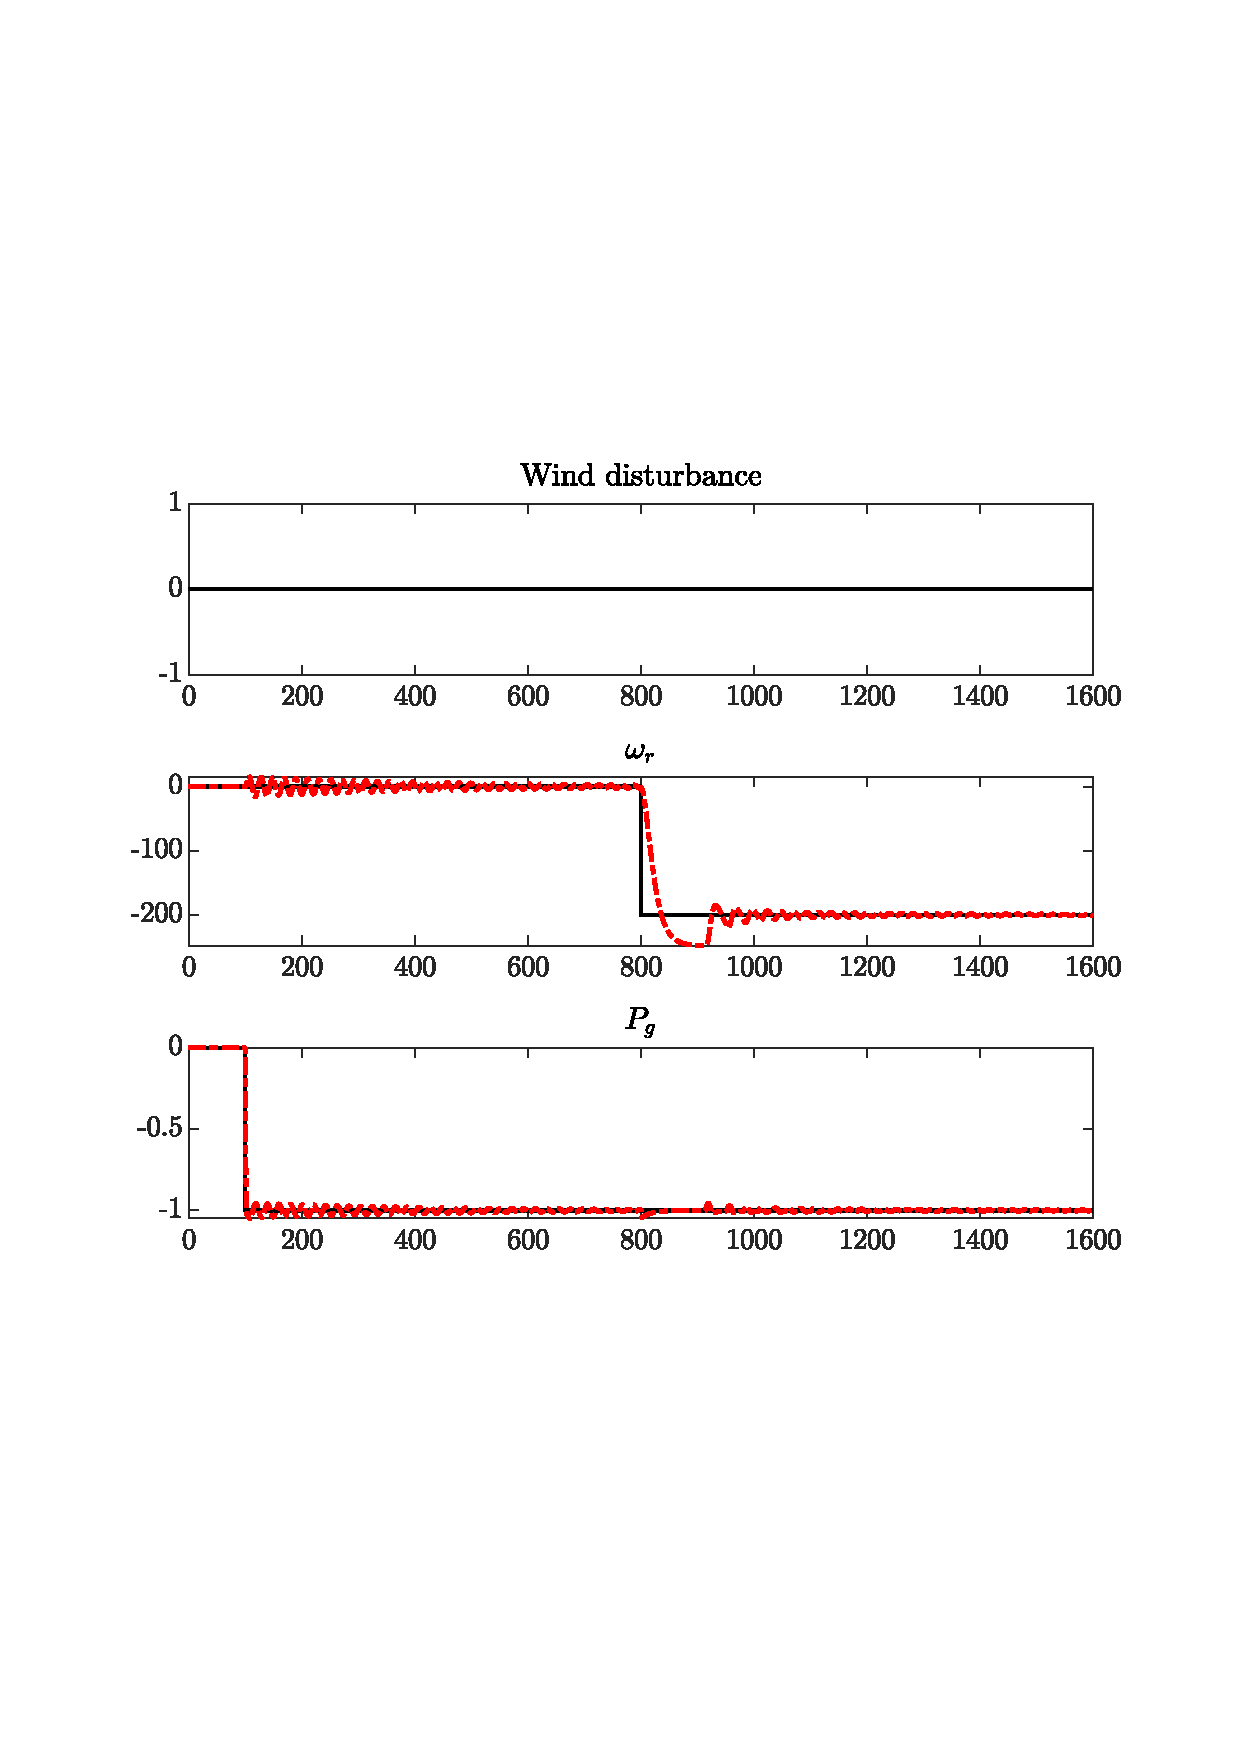
\includegraphics[width=1\linewidth, scale=1, trim=55 230 55 120,clip]{fig/Open_loop/exp_1_ref.pdf}}
%
    \subcaptionbox{Blade pitch angle and duty cycle over time before and after saturation. \label{fig:app:cl_results:exp1:in}}[.45\textwidth]{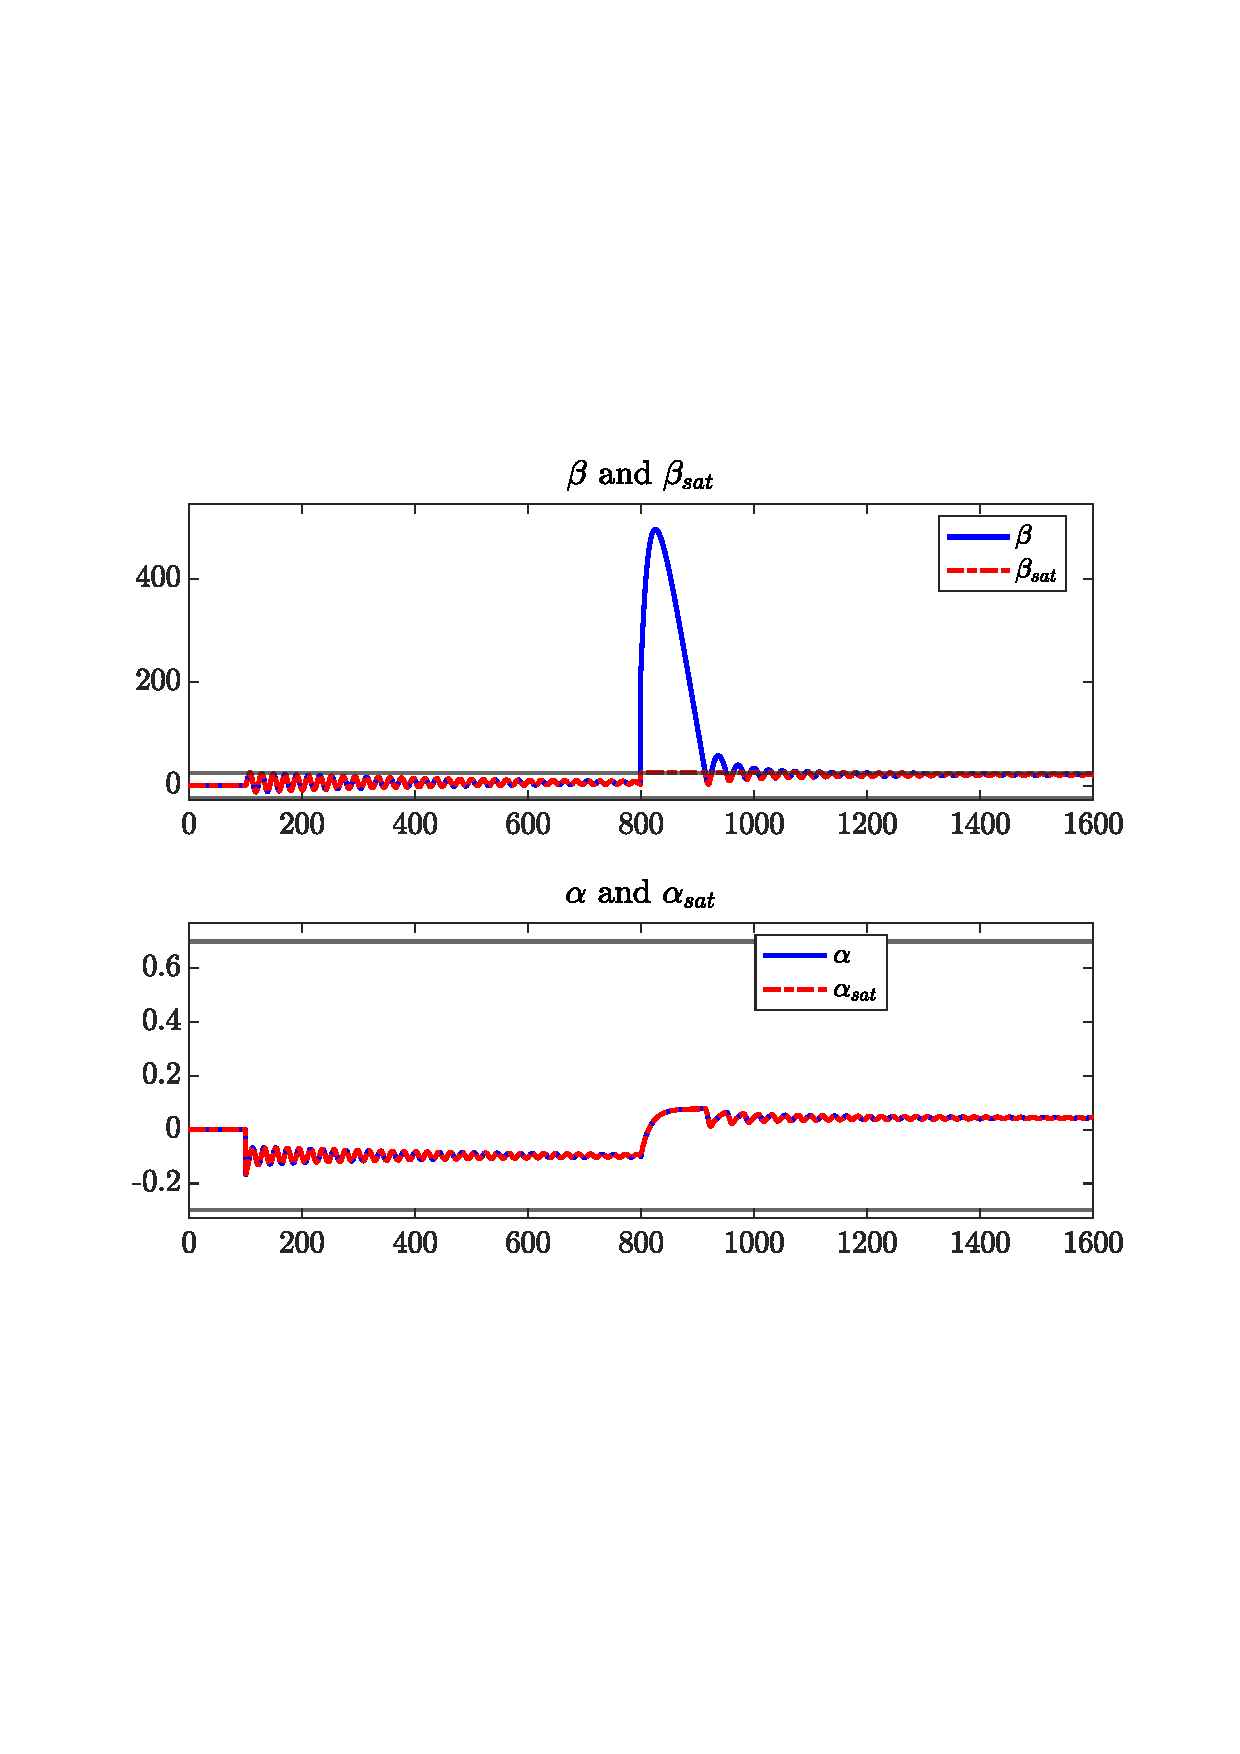
\includegraphics[width=1\linewidth, scale=1, trim=55 230 55 120,clip]{fig/Open_loop/exp_1_in.pdf}}
\\
\subcaptionbox{Relative error over time. \label{fig:app:cl_results:exp1:error}}[.7\textwidth]{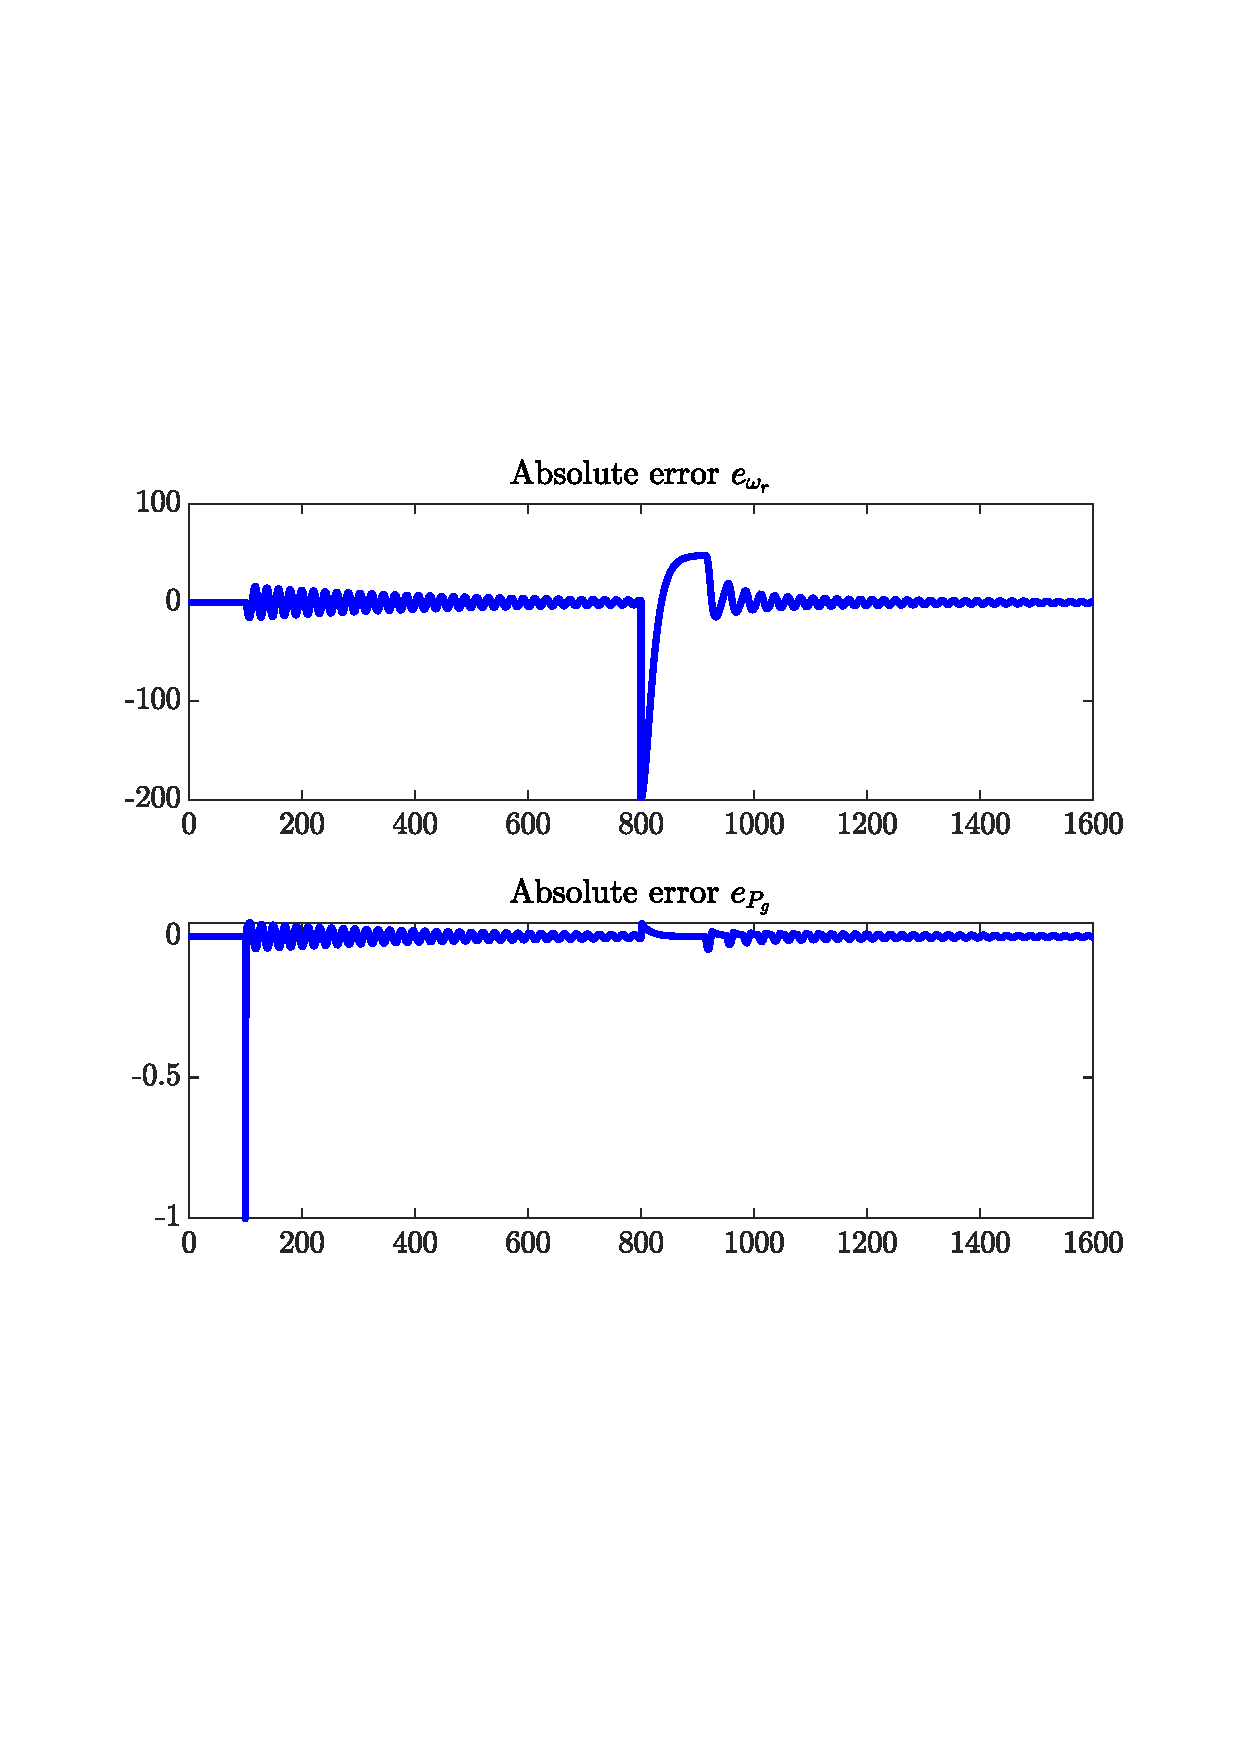
\includegraphics[width=1\linewidth, scale=1, trim=55 230 55 120,clip]{fig/Open_loop/exp_1_error.pdf}}
    \caption{Visualization of reference signal, the controller output and the absolute error}
    \label{fig:app:cl_results:exp1}
\end{figure}




\subsection{Experiment 2}

\begin{figure}[H]
    \centering

    \subcaptionbox{Wind disturbance, rotational speed of blade and power consumption over time \label{fig:app:cl_results:exp2:ref}}[.45\textwidth]{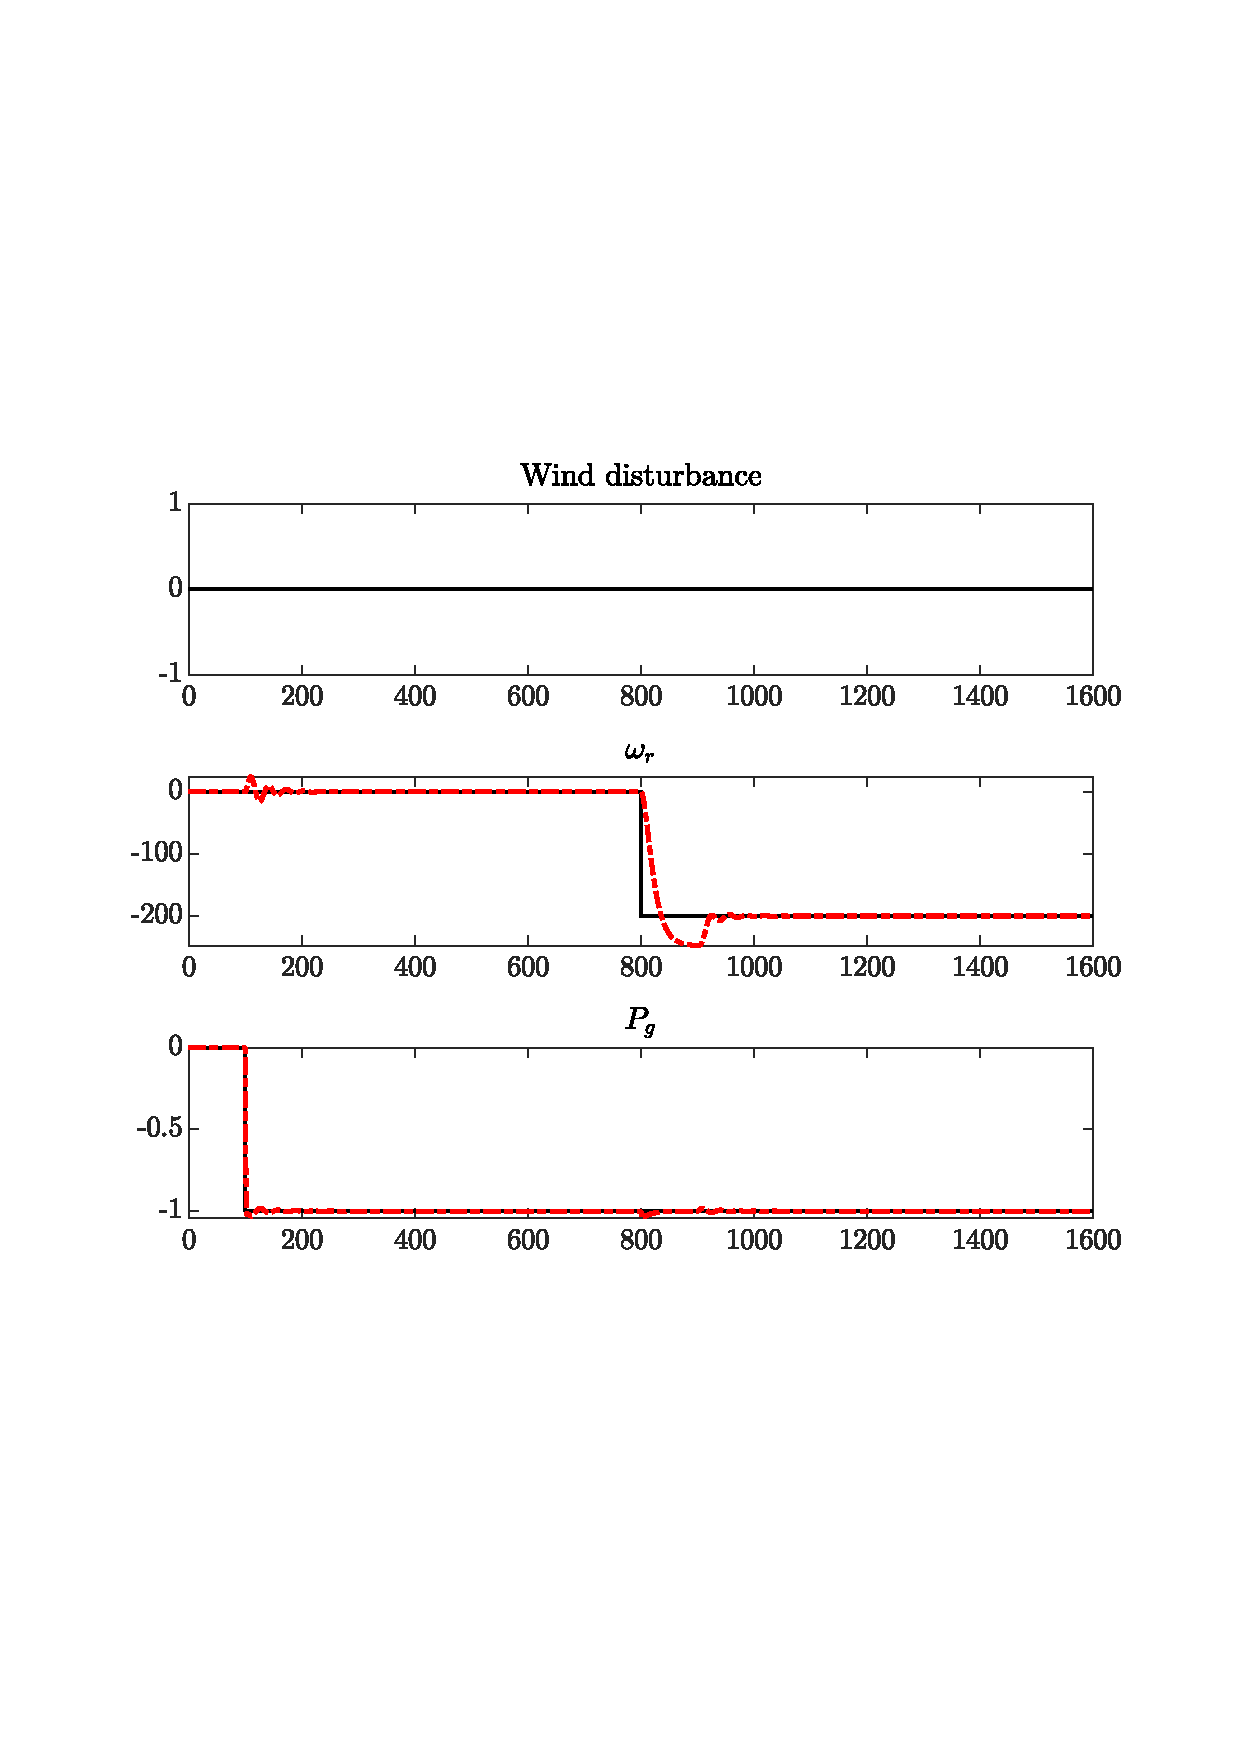
\includegraphics[width=1\linewidth, scale=1, trim=55 230 55 120,clip]{fig/Open_loop/exp_2_ref.pdf}}
%
    \subcaptionbox{Blade pitch angle and duty cycle over time before and after saturation. \label{fig:app:cl_results:exp2:in}}[.45\textwidth]{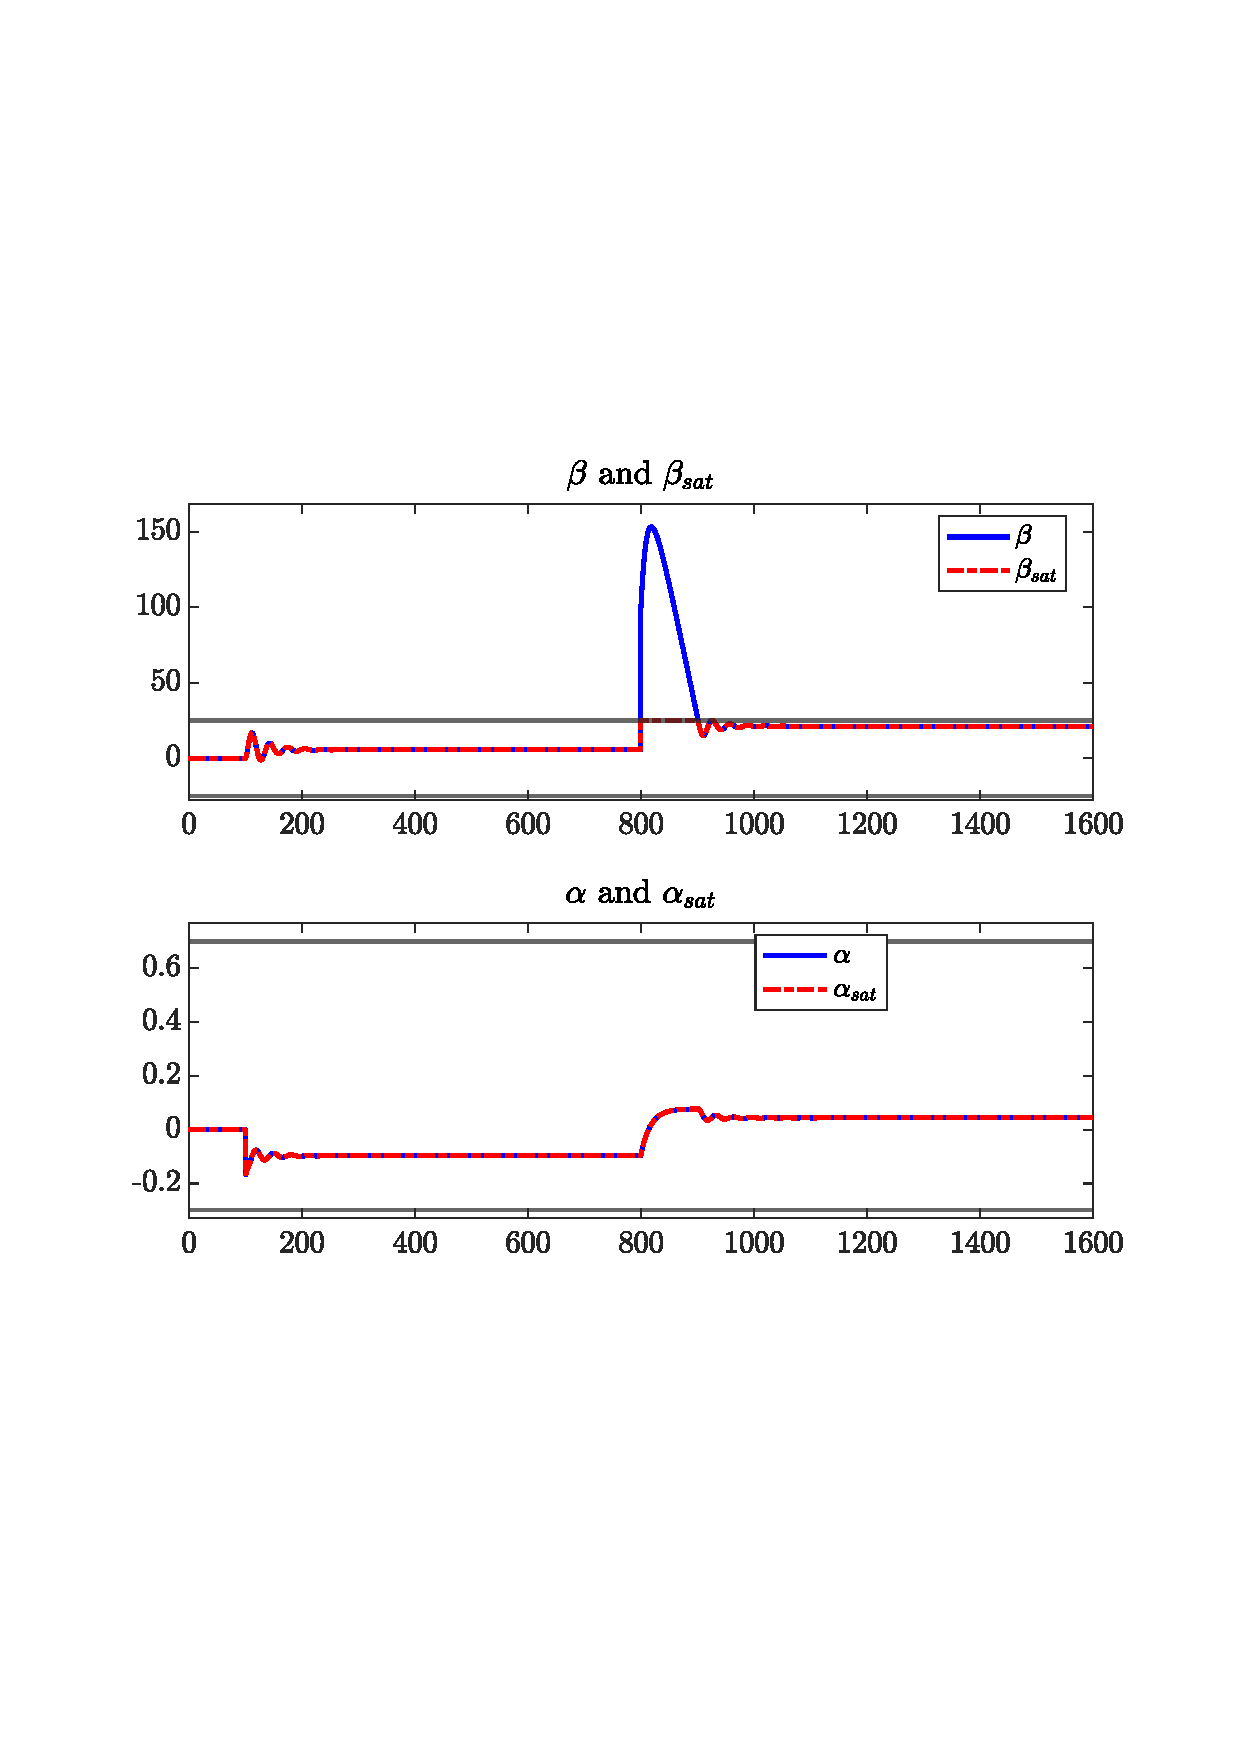
\includegraphics[width=1\linewidth, scale=1, trim=55 230 55 120,clip]{fig/Open_loop/exp_2_in.pdf}}
\\
\subcaptionbox{Relative error over time. \label{fig:app:cl_results:exp2:error}}[.7\textwidth]{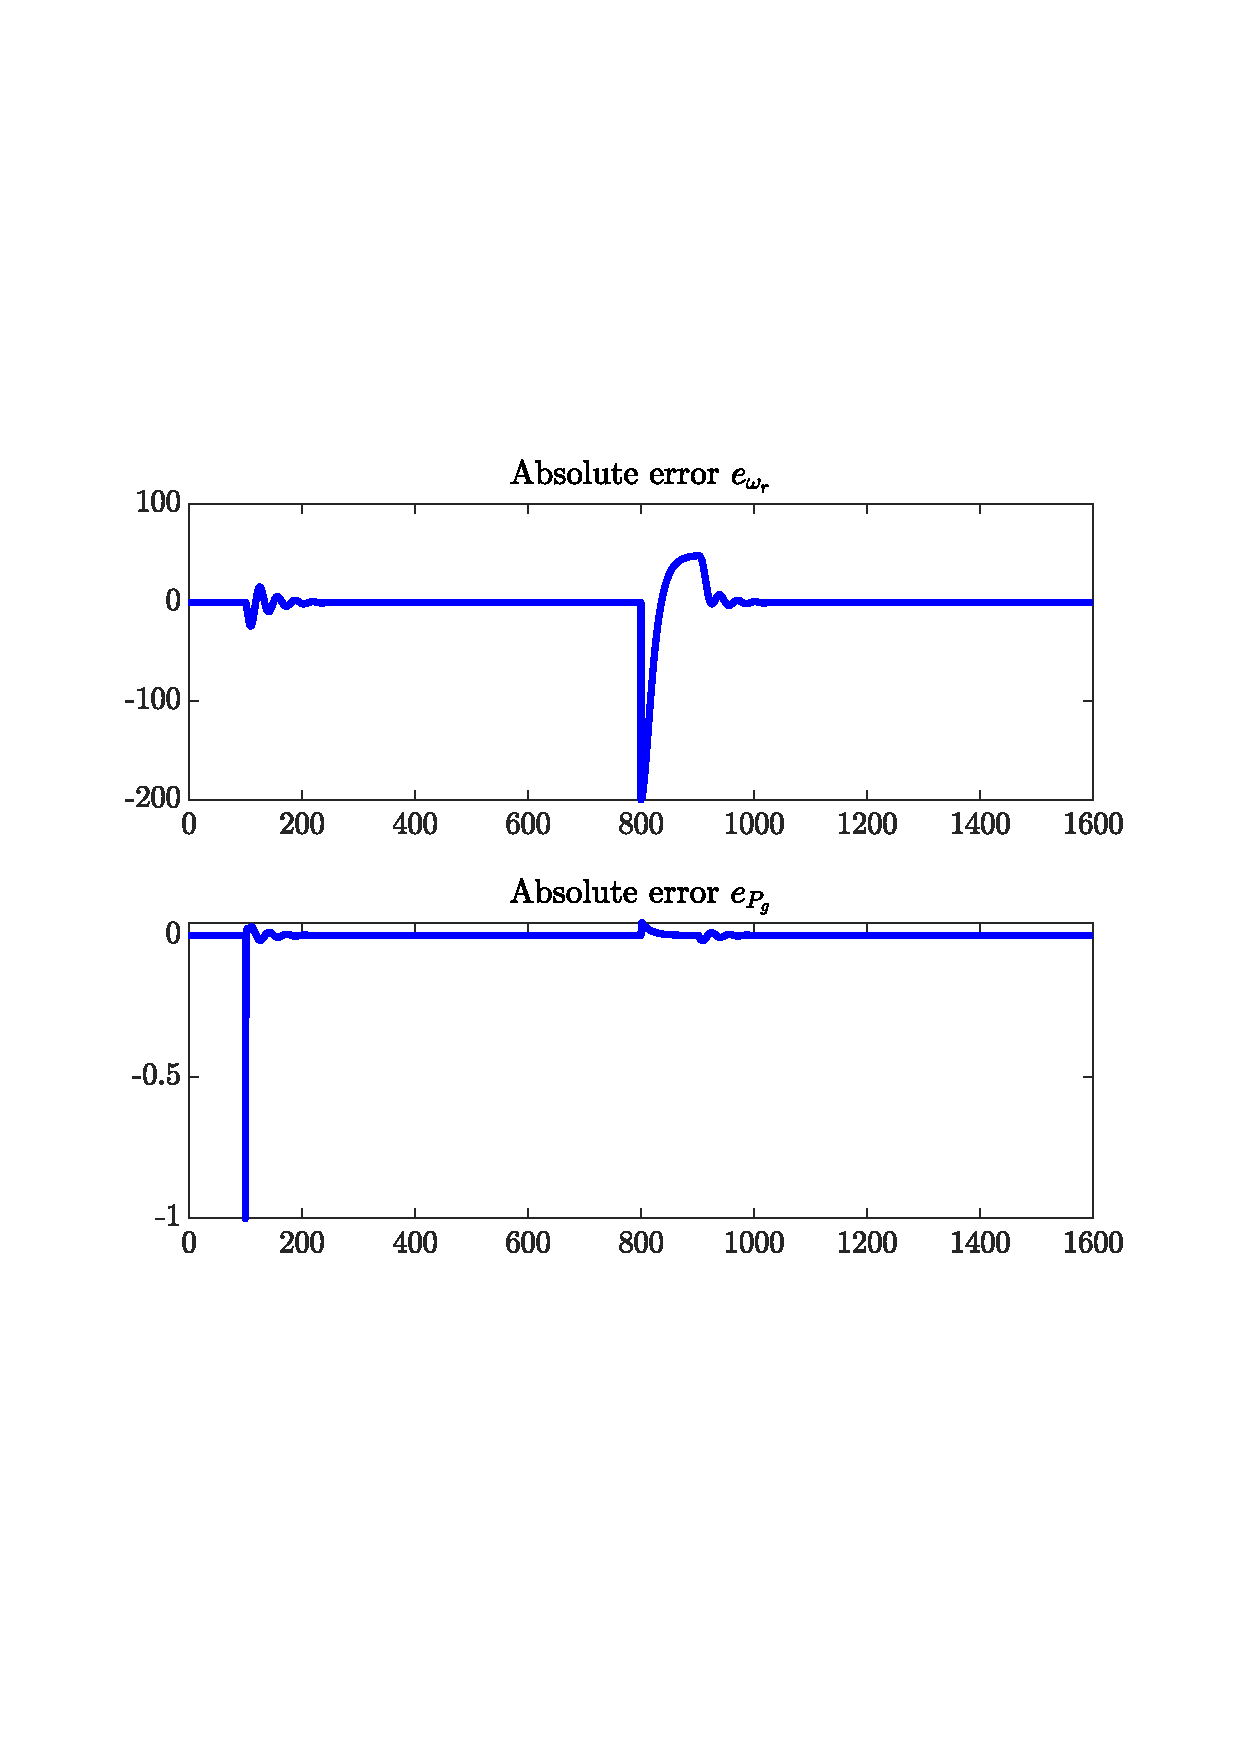
\includegraphics[width=1\linewidth, scale=1, trim=55 230 55 120,clip]{fig/Open_loop/exp_2_error.pdf}}
    \caption{Visualization of reference signal, the controller output and the absolute error}
    \label{fig:app:cl_results:exp2}
\end{figure}


\subsection{Experiment 3}

\begin{figure}[H]
    \centering

    \subcaptionbox{Wind disturbance, rotational speed of blade and power consumption over time \label{fig:app:cl_results:exp3:ref}}[.45\textwidth]{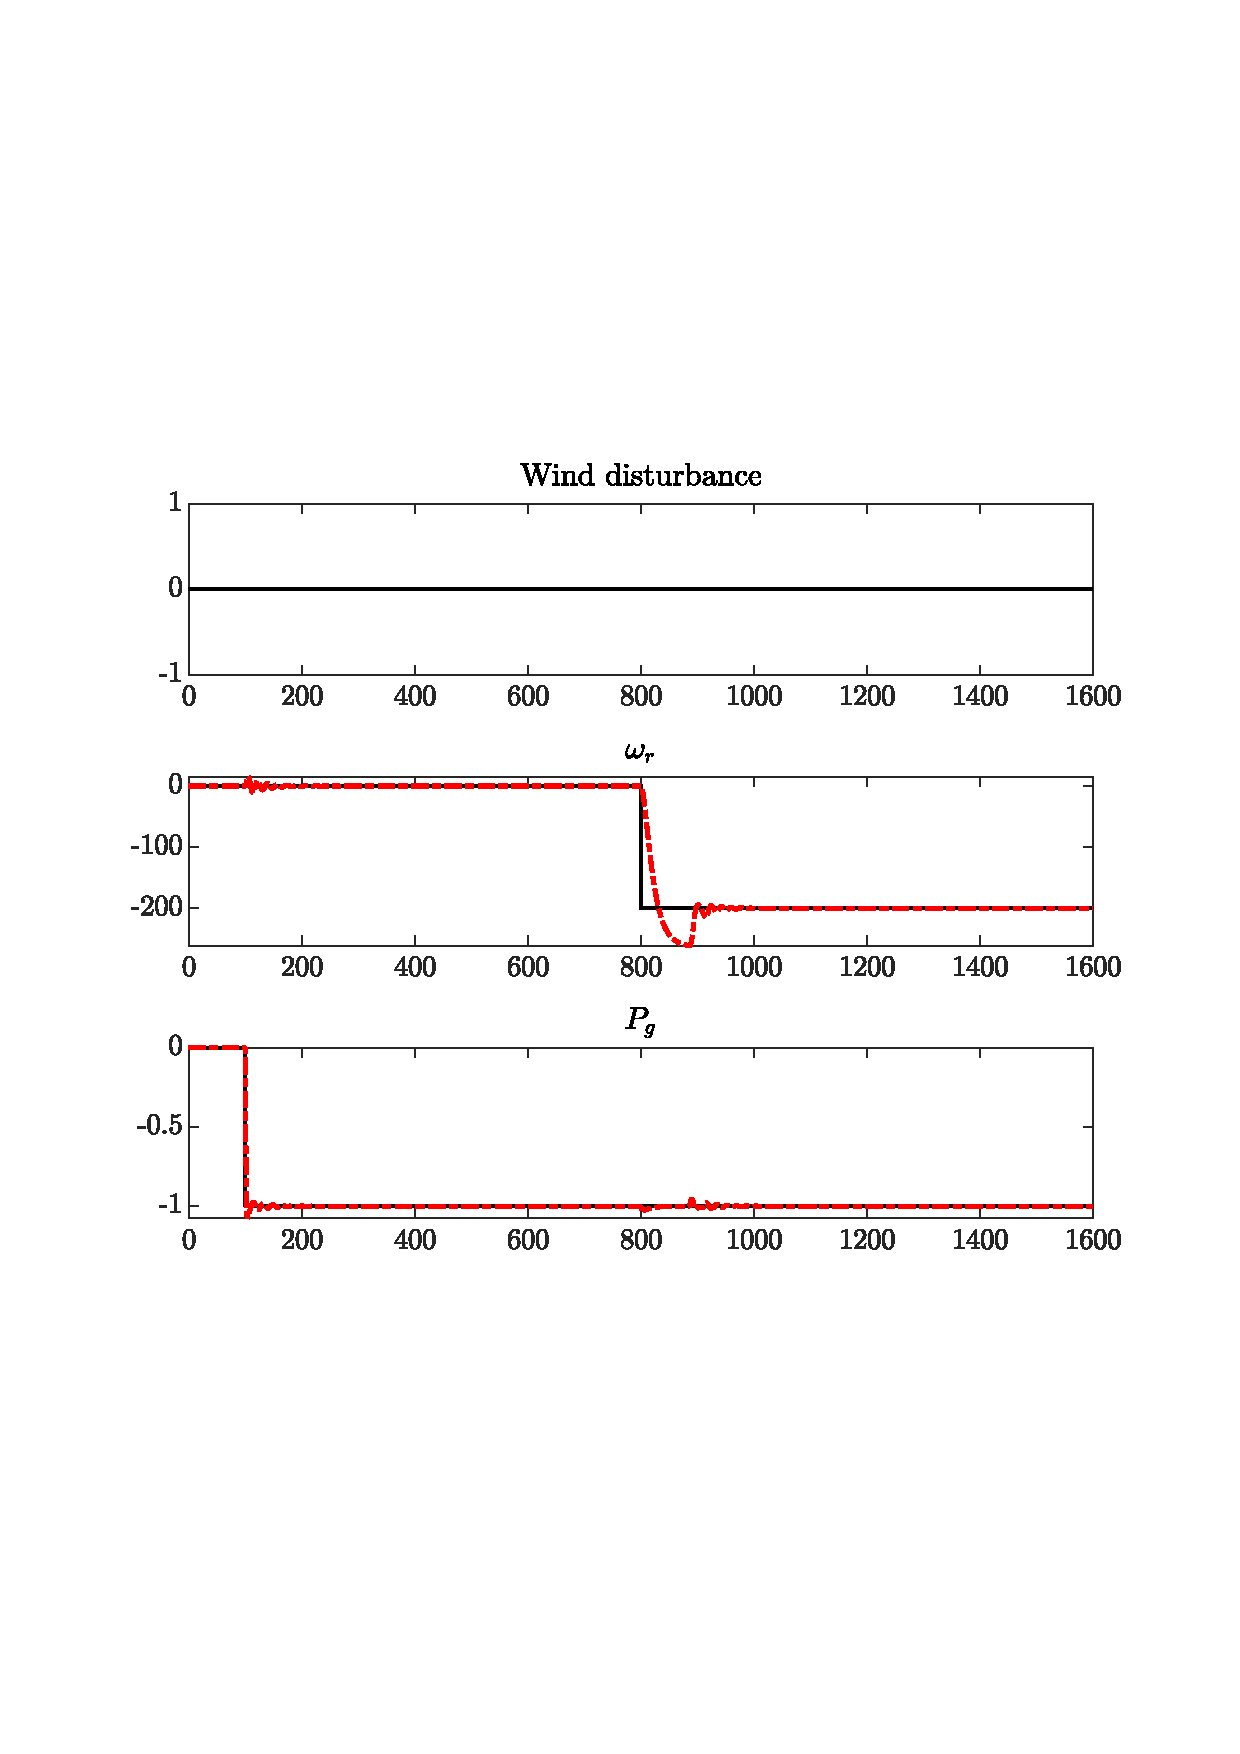
\includegraphics[width=1\linewidth, scale=1, trim=55 230 55 120,clip]{fig/Open_loop/exp_3_ref.pdf}}
%
    \subcaptionbox{Blade pitch angle and duty cycle over time before and after saturation. \label{fig:app:cl_results:exp3:in}}[.45\textwidth]{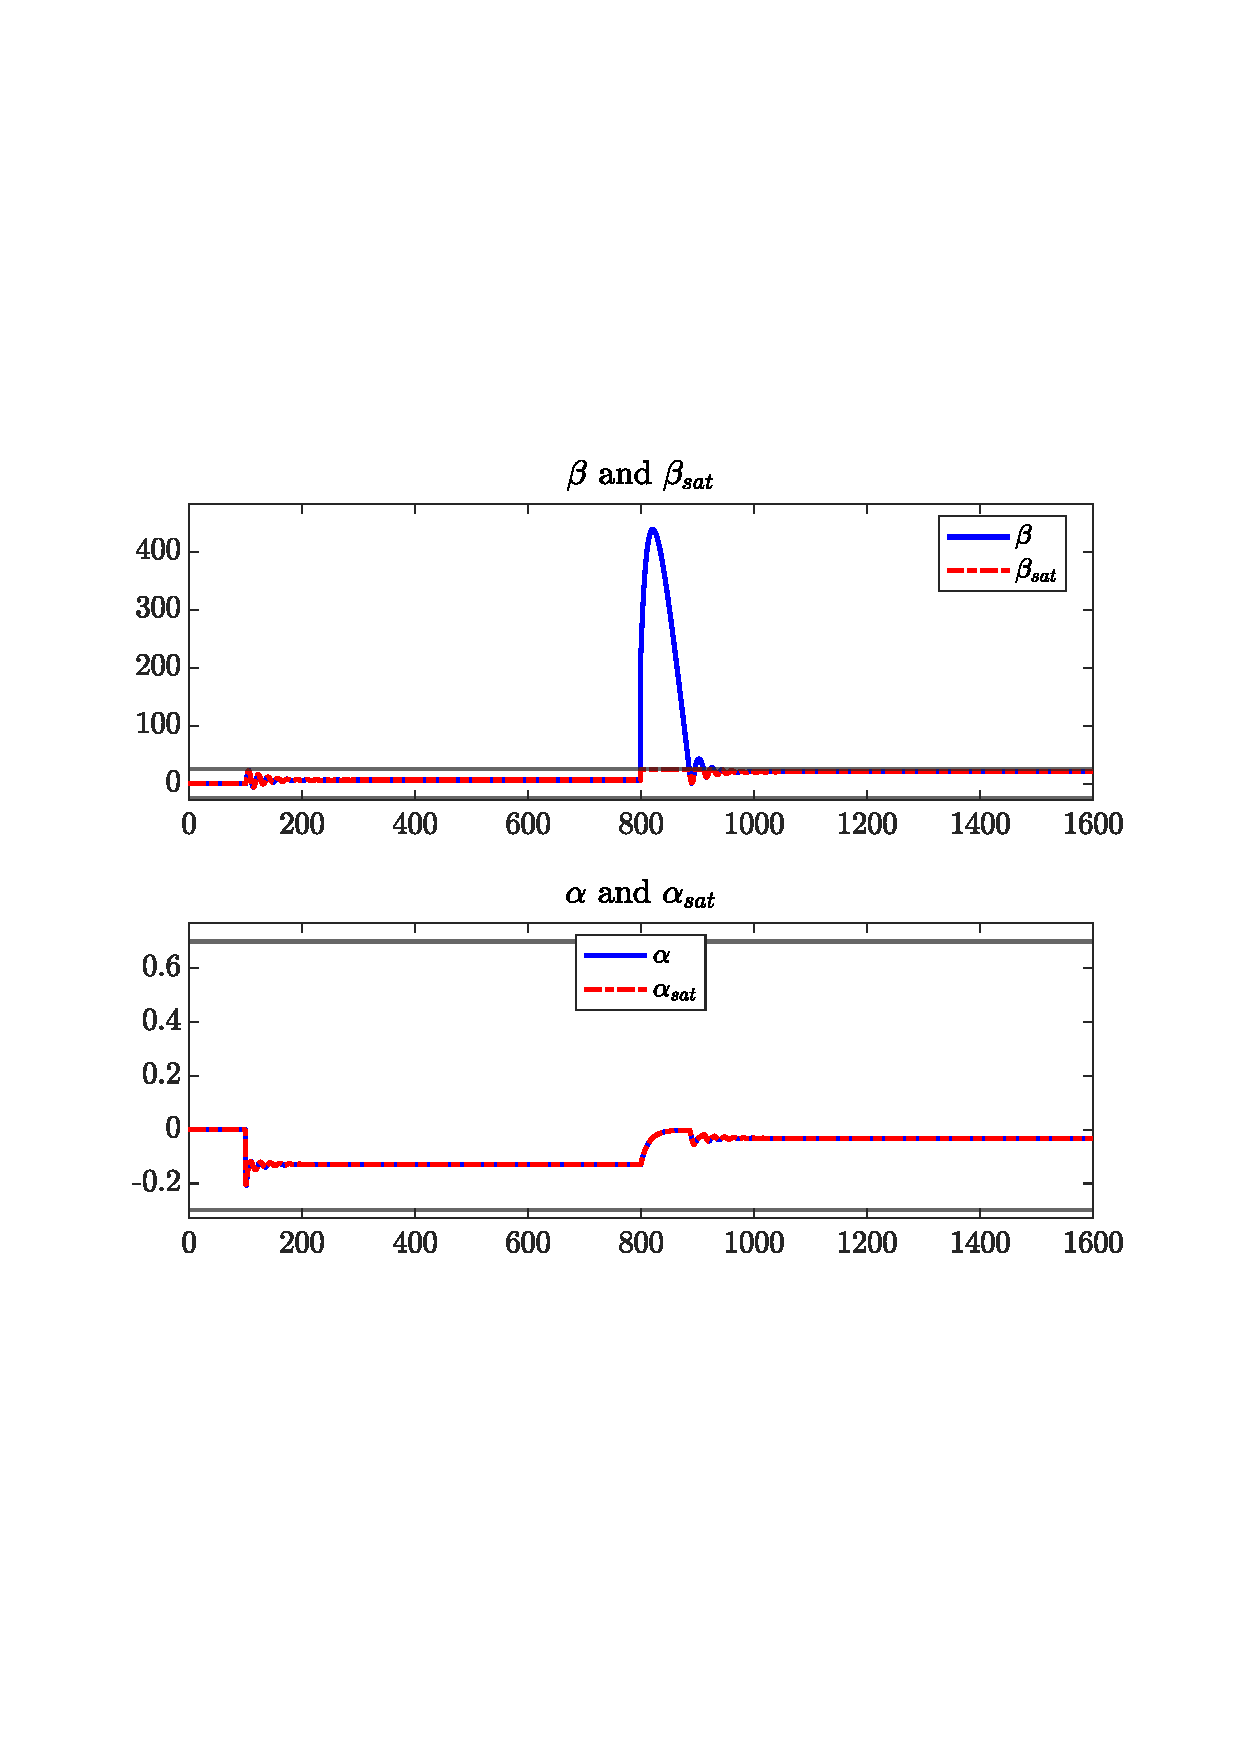
\includegraphics[width=1\linewidth, scale=1, trim=55 230 55 120,clip]{fig/Open_loop/exp_3_in.pdf}}
\\
\subcaptionbox{Relative error over time. \label{fig:app:cl_results:exp3:error}}[.7\textwidth]{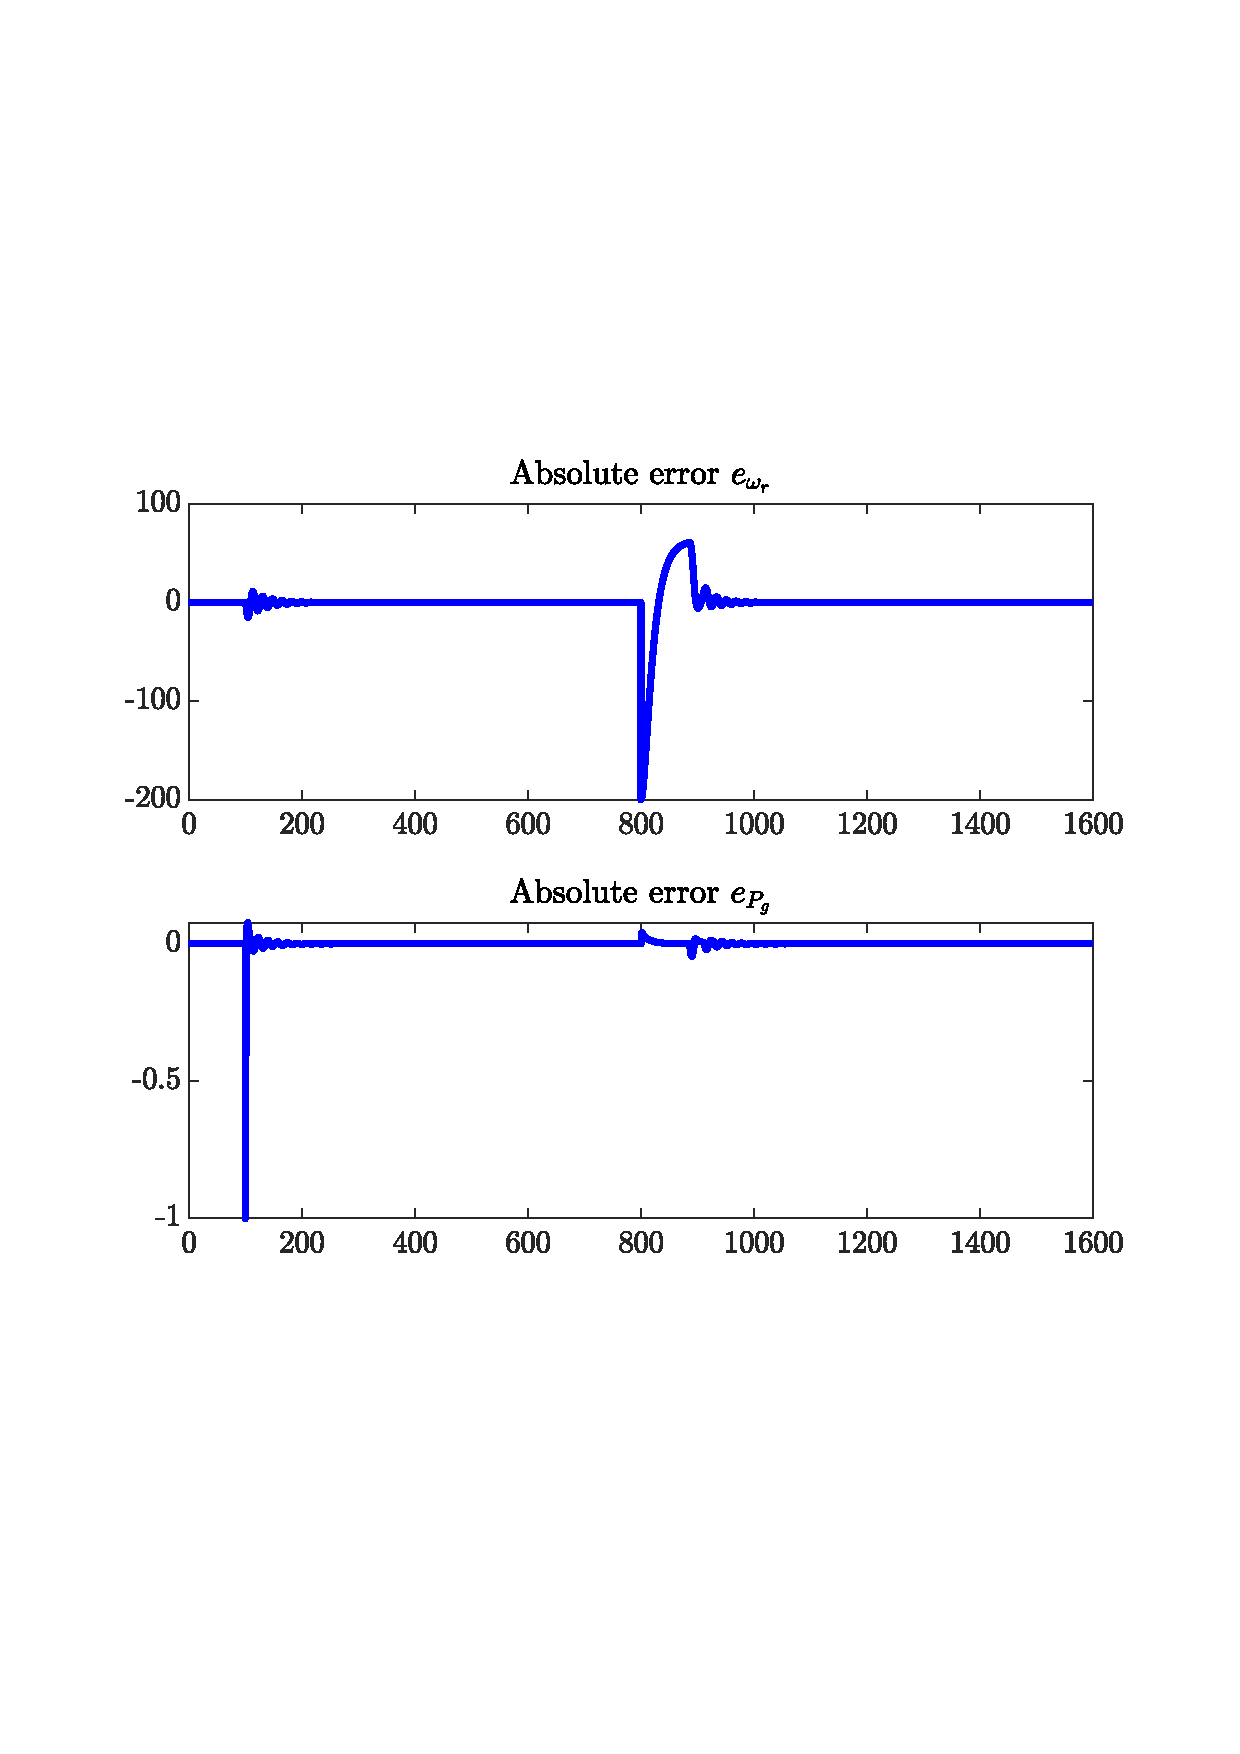
\includegraphics[width=1\linewidth, scale=1, trim=55 230 55 120,clip]{fig/Open_loop/exp_3_error.pdf}}
    \caption{Visualization of reference signal, the controller output and the absolute error}
    \label{fig:app:cl_results:exp3}
\end{figure}

\subsection{Experiment 4}

\begin{figure}[H]
    \centering

    \subcaptionbox{Wind disturbance, rotational speed of blade and power consumption over time \label{fig:app:cl_results:exp4:ref}}[.45\textwidth]{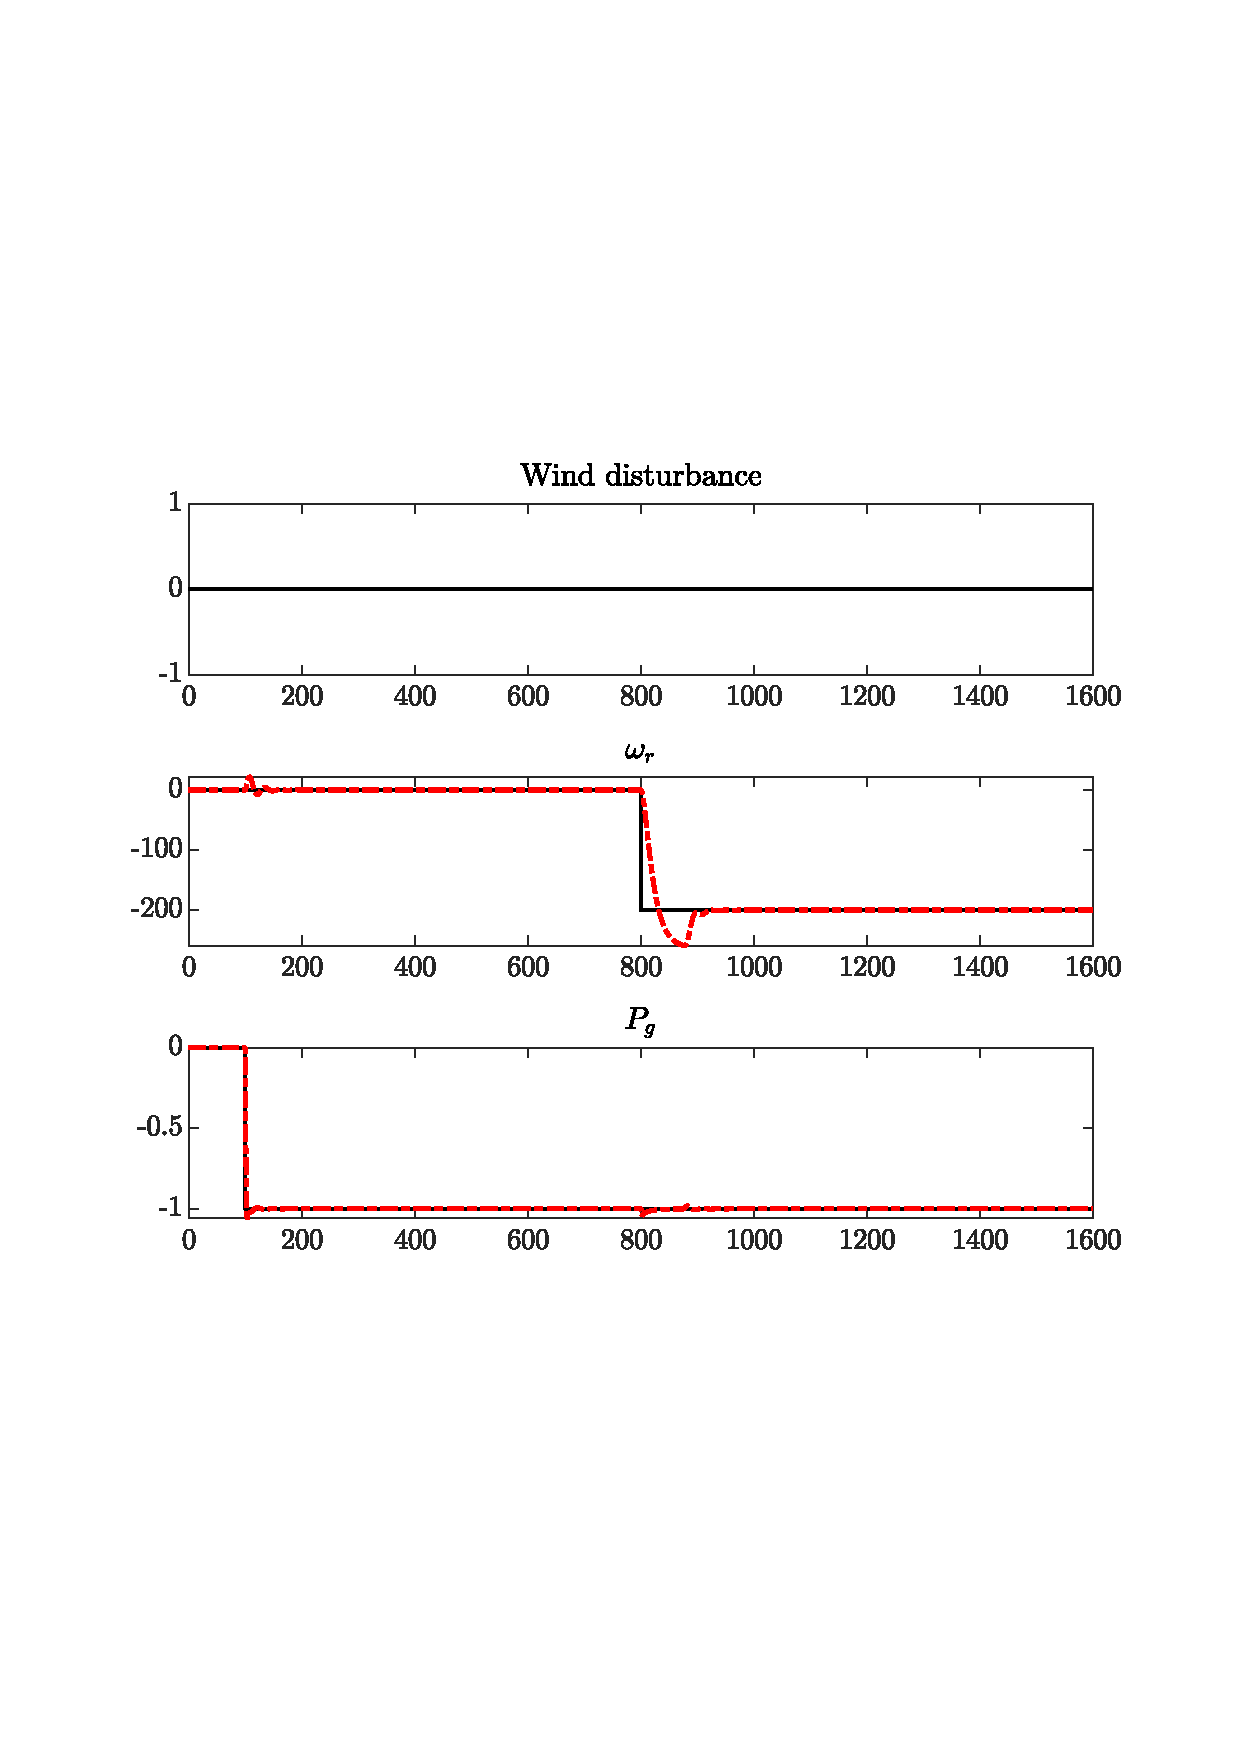
\includegraphics[width=1\linewidth, scale=1, trim=55 230 55 120,clip]{fig/Open_loop/exp_4_ref.pdf}}
%
    \subcaptionbox{Blade pitch angle and duty cycle over time before and after saturation. \label{fig:app:cl_results:exp4:in}}[.45\textwidth]{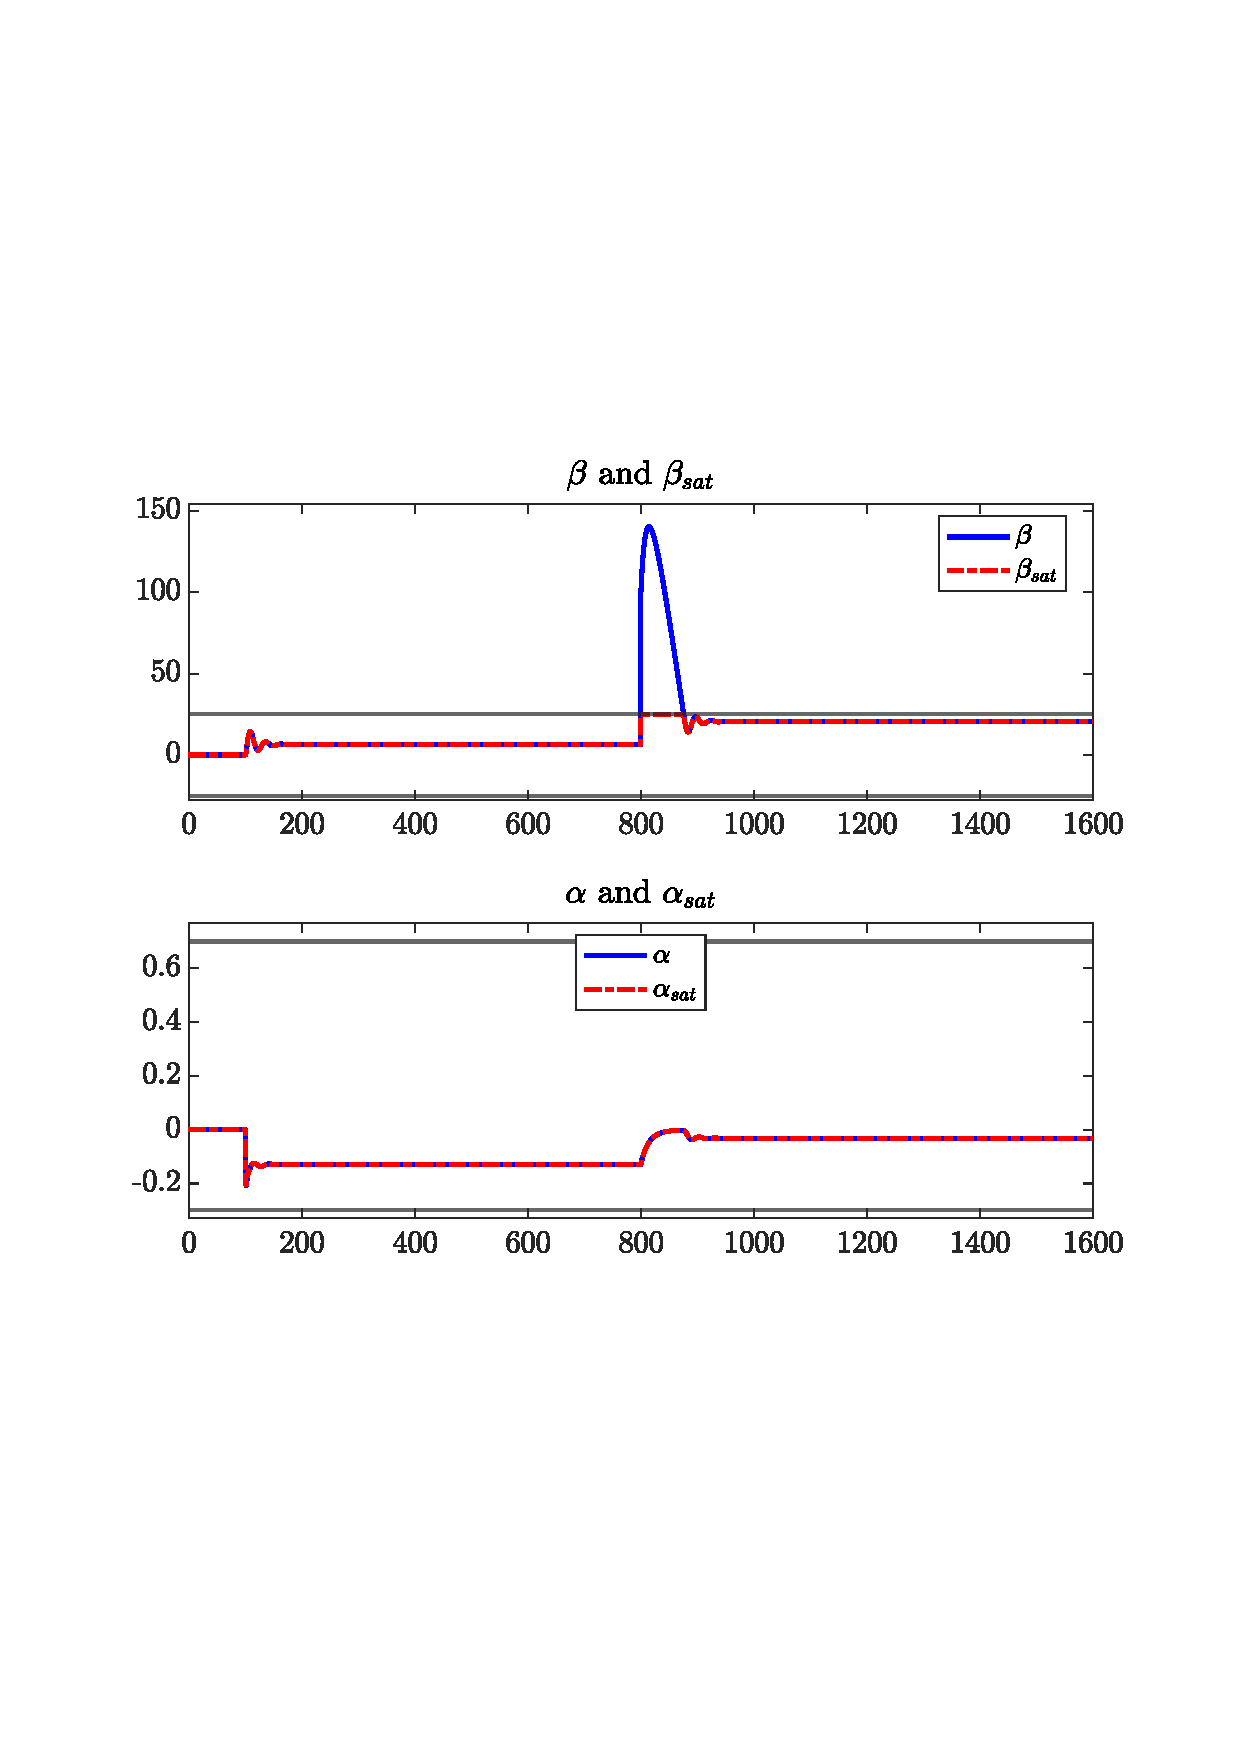
\includegraphics[width=1\linewidth, scale=1, trim=55 230 55 120,clip]{fig/Open_loop/exp_4_in.pdf}}
\\
\subcaptionbox{Relative error over time. \label{fig:app:cl_results:exp4:error}}[.7\textwidth]{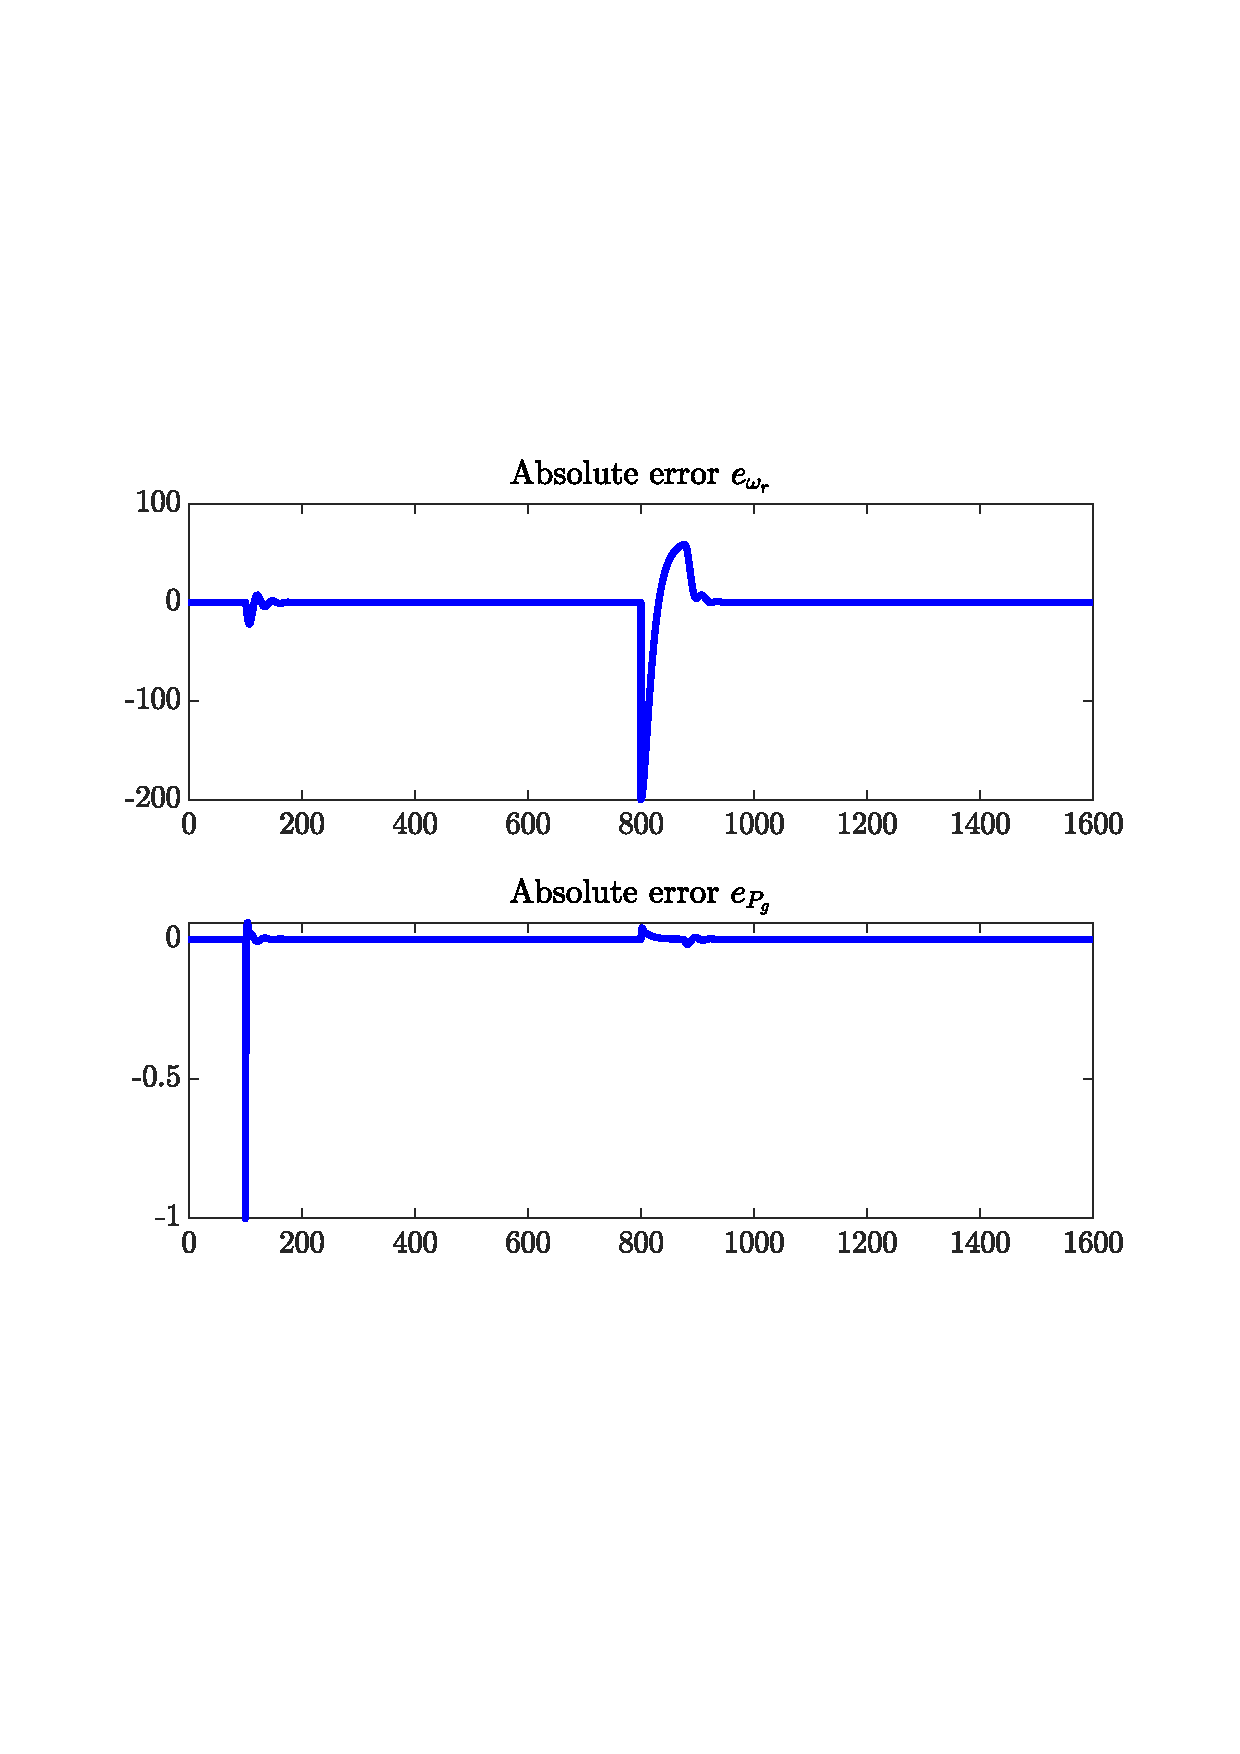
\includegraphics[width=1\linewidth, scale=1, trim=55 230 55 120,clip]{fig/Open_loop/exp_4_error.pdf}}
    \caption{Visualization of reference signal, the controller output and the absolute error}
    \label{fig:app:cl_results:exp4}
\end{figure}


\subsection{Experiment 5}

\begin{figure}[H]
    \centering

    \subcaptionbox{Wind disturbance, rotational speed of blade and power consumption over time \label{fig:app:cl_results:exp5:ref}}[.45\textwidth]{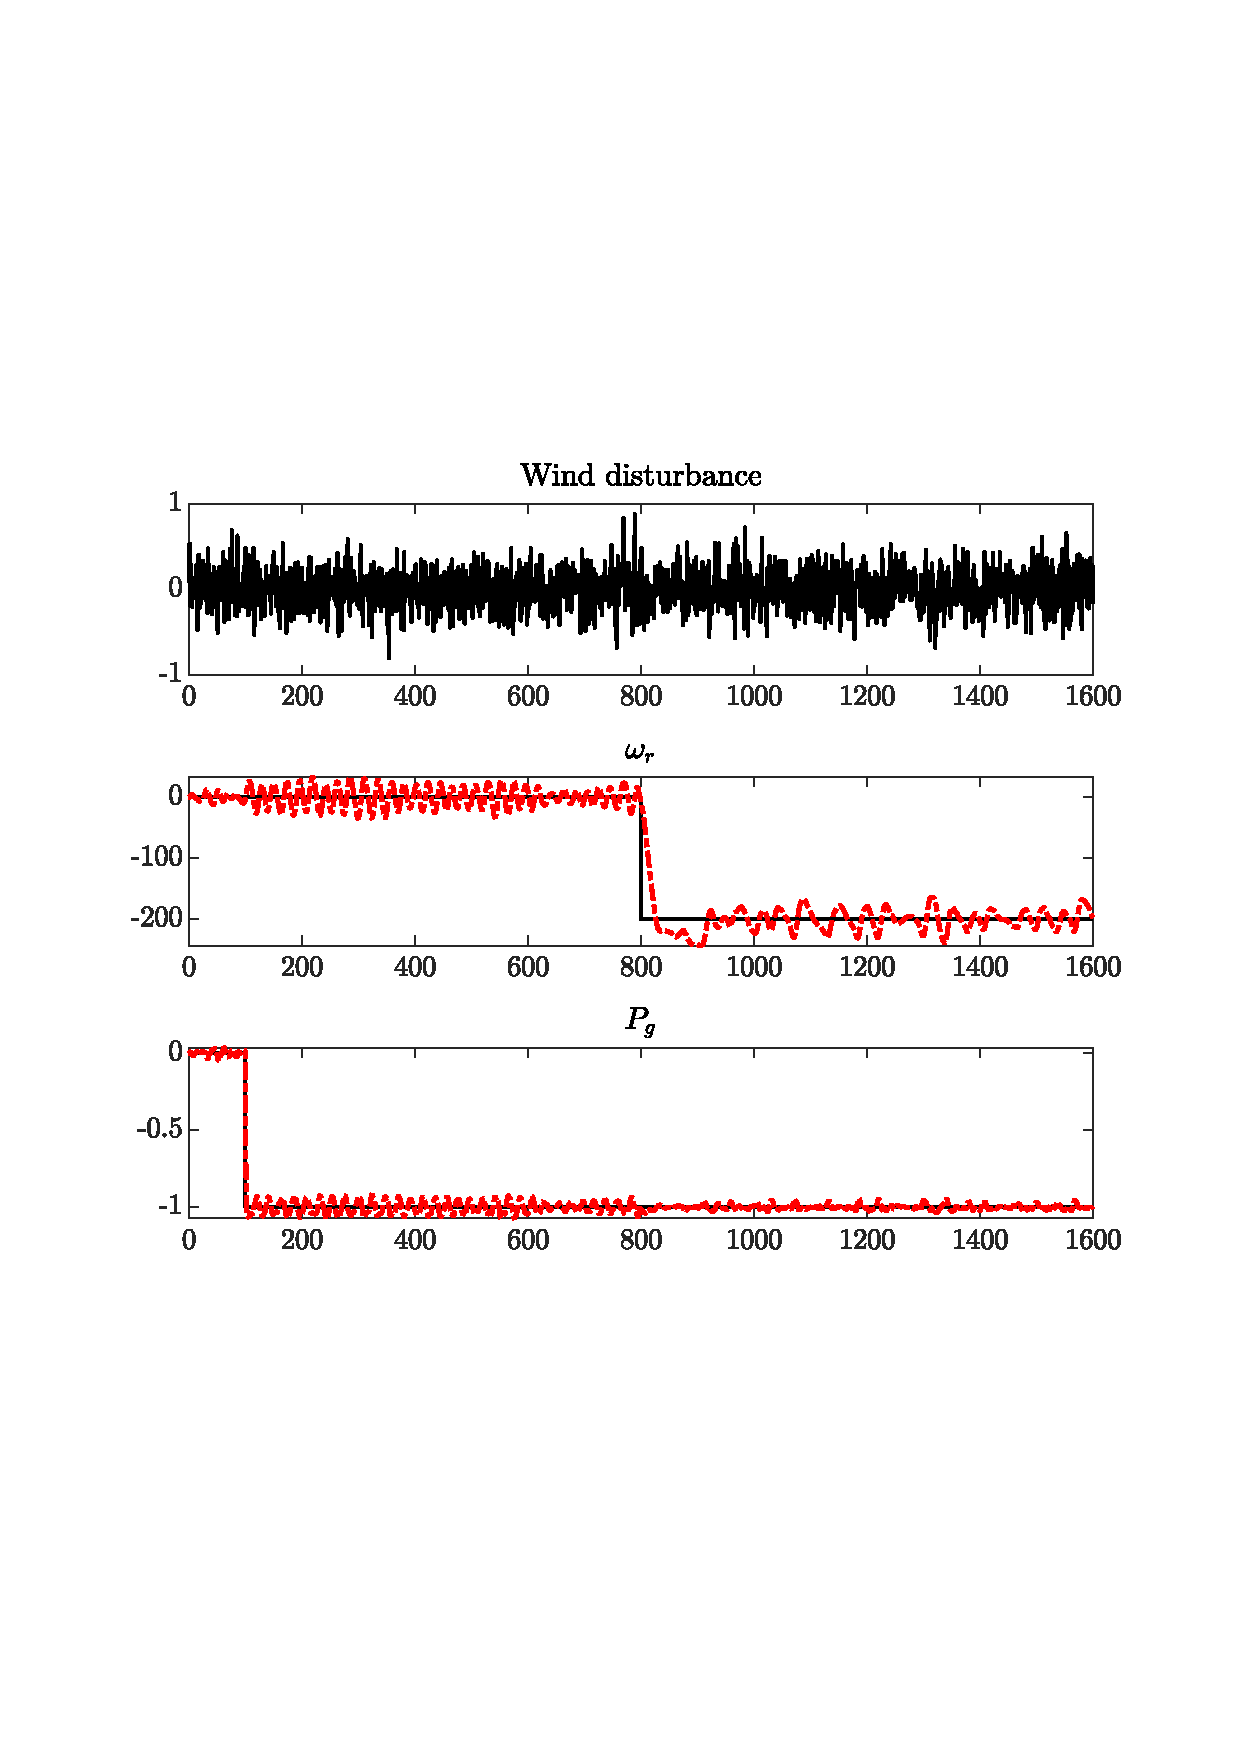
\includegraphics[width=1\linewidth, scale=1, trim=55 230 55 120,clip]{fig/Open_loop/exp_5_ref.pdf}}
%
    \subcaptionbox{Blade pitch angle and duty cycle over time before and after saturation. \label{fig:app:cl_results:exp5:in}}[.45\textwidth]{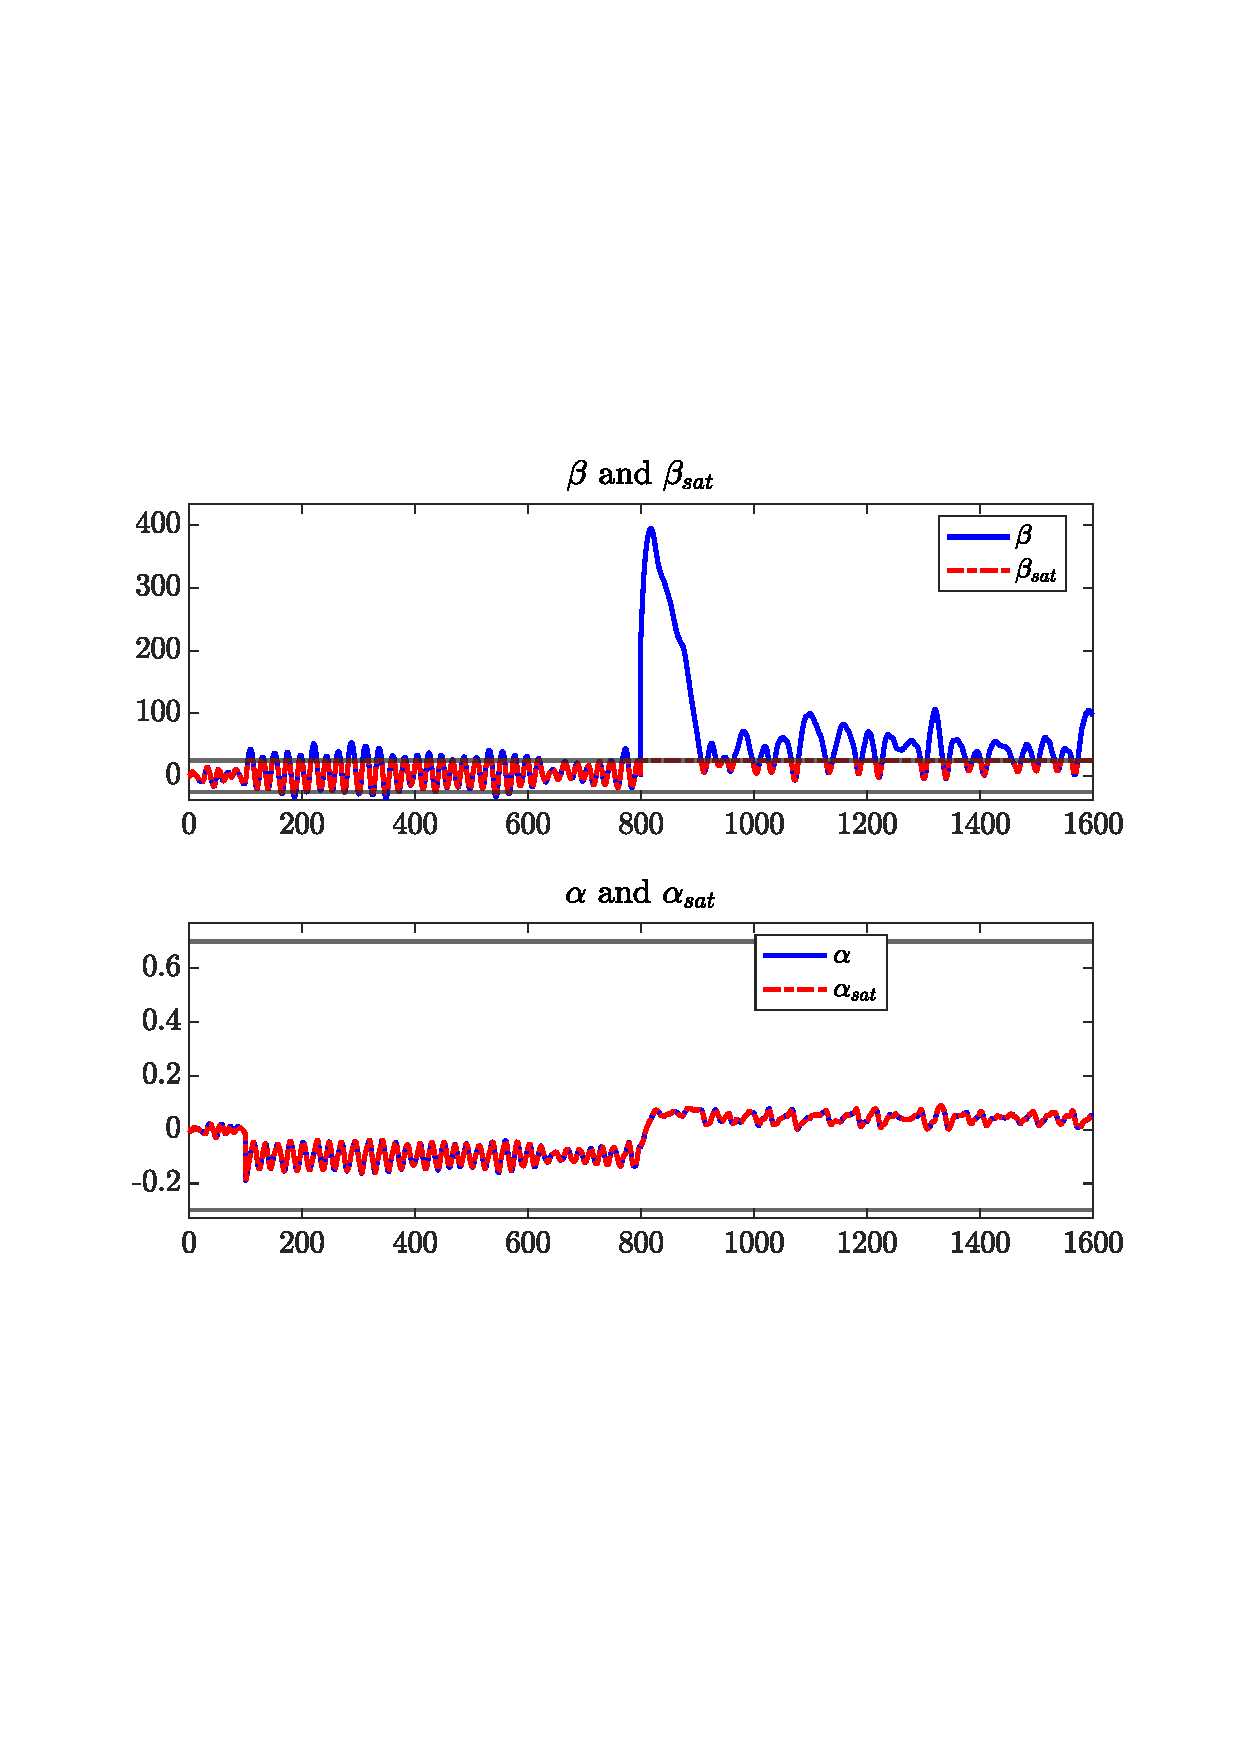
\includegraphics[width=1\linewidth, scale=1, trim=55 230 55 120,clip]{fig/Open_loop/exp_5_in.pdf}}
\\
\subcaptionbox{Relative error over time. \label{fig:app:cl_results:exp5:error}}[.7\textwidth]{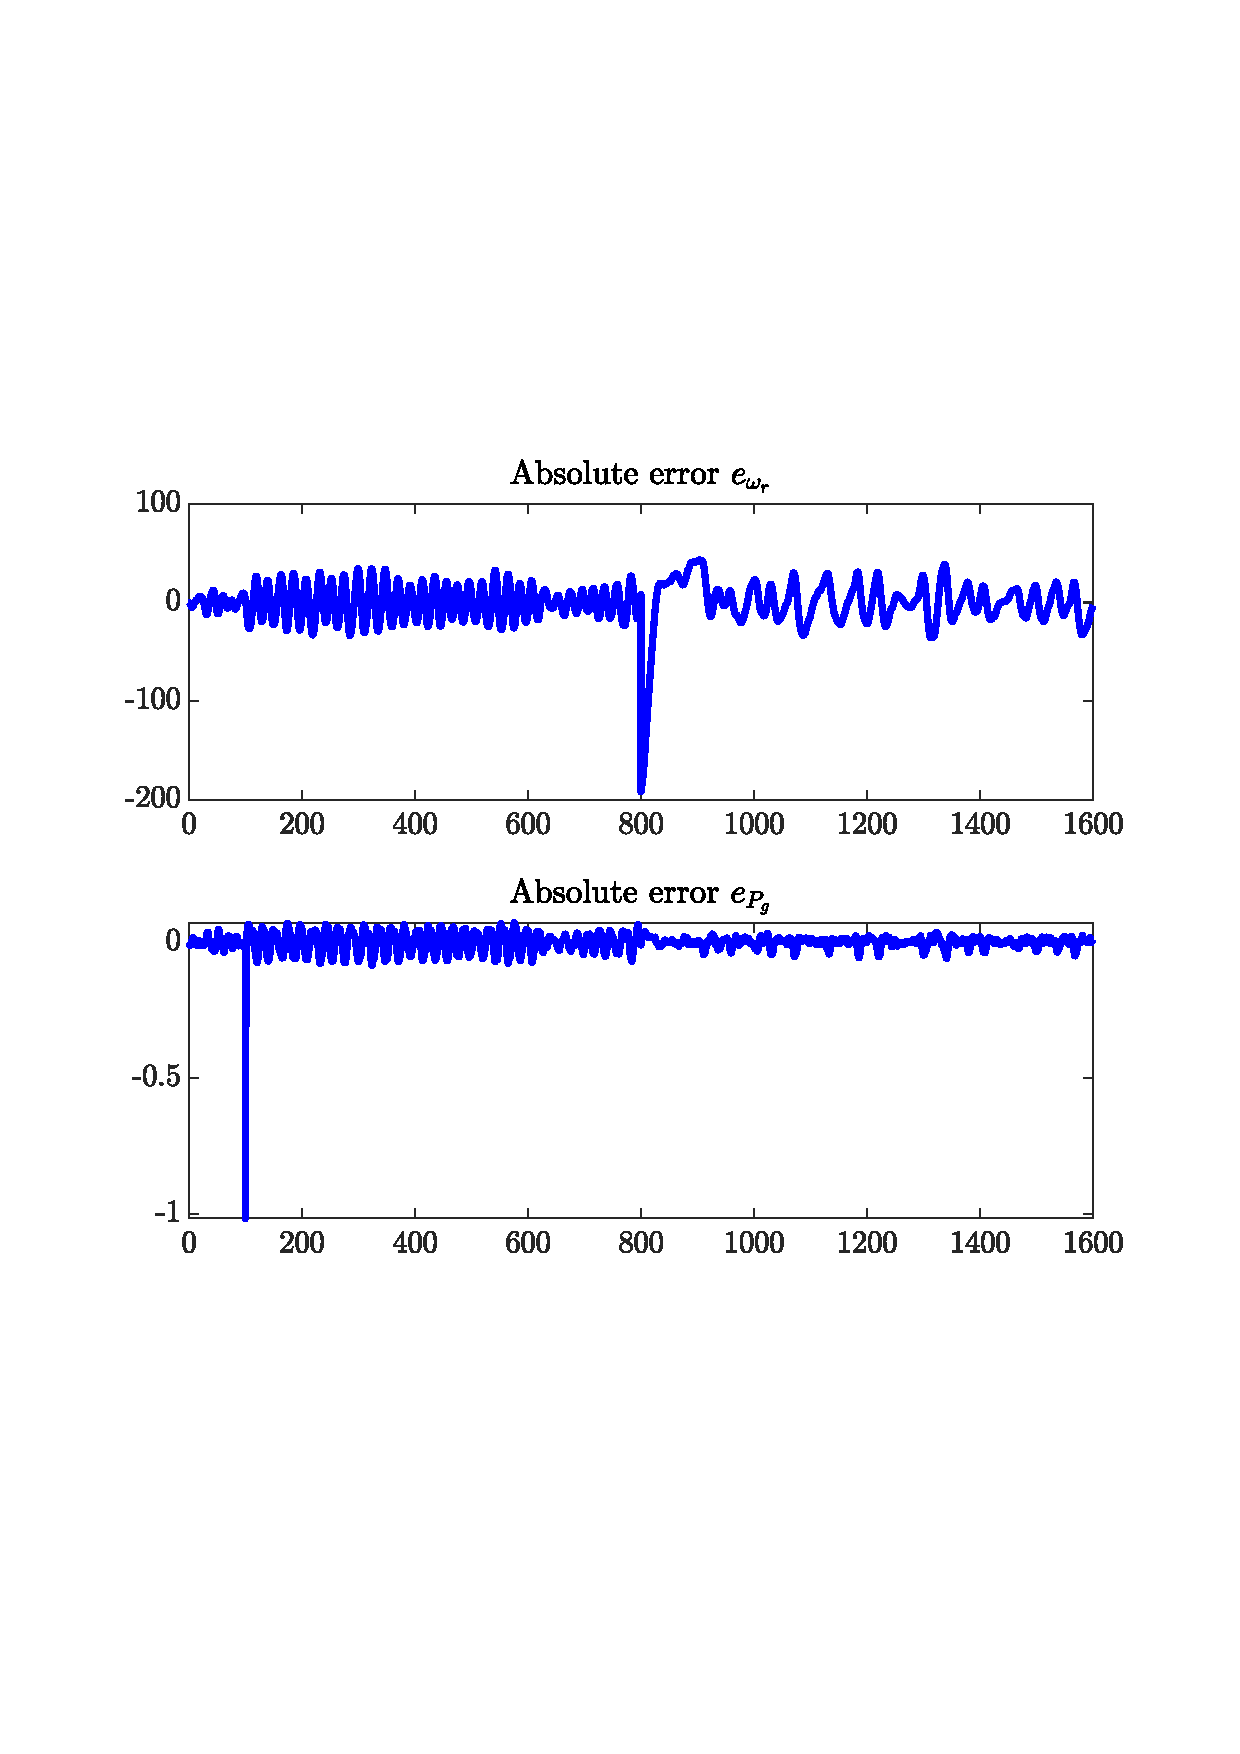
\includegraphics[width=1\linewidth, scale=1, trim=55 230 55 120,clip]{fig/Open_loop/exp_5_error.pdf}}
    \caption{Visualization of reference signal, the controller output and the absolute error}
    \label{fig:app:cl_results:exp5}
\end{figure}

\subsection{Experiment 6}

\begin{figure}[H]
    \centering

    \subcaptionbox{Wind disturbance, rotational speed of blade and power consumption over time \label{fig:app:cl_results:exp6:ref}}[.45\textwidth]{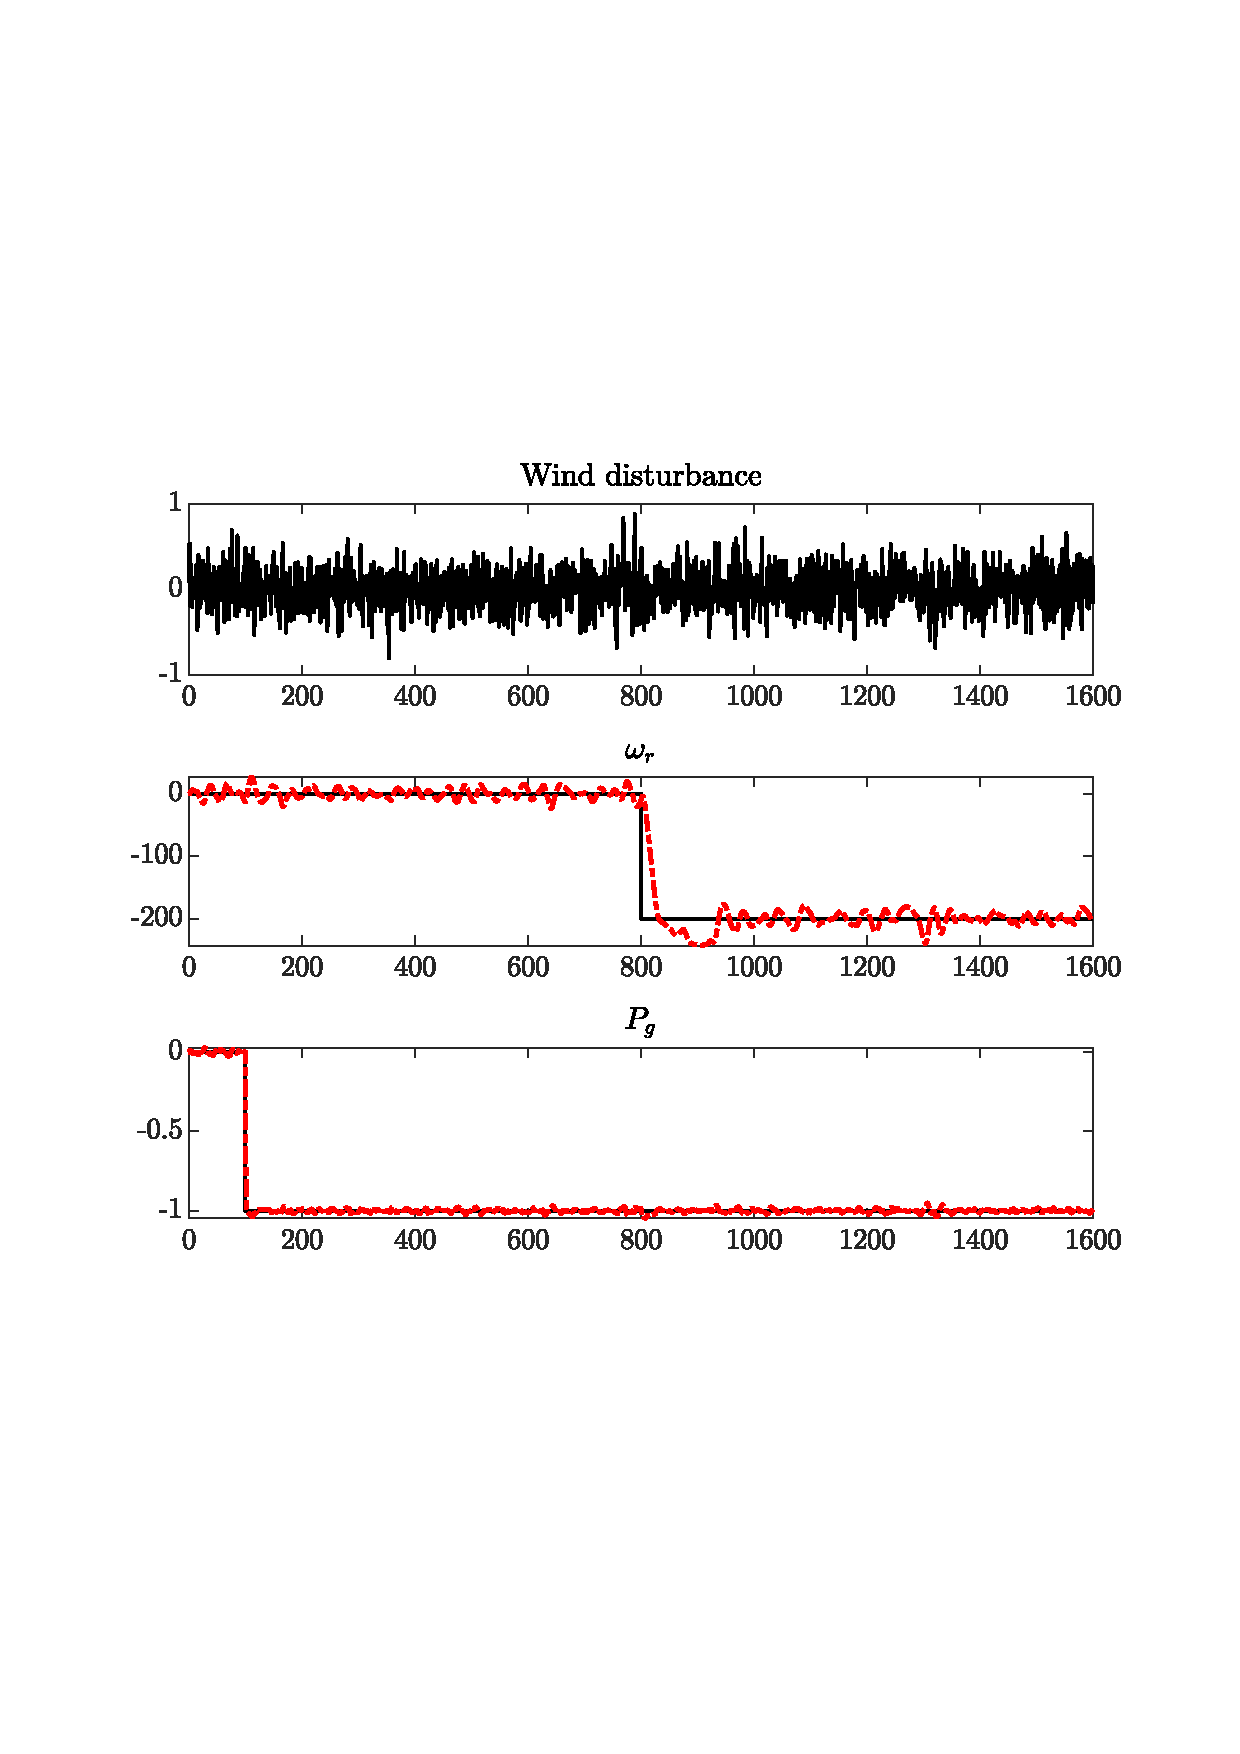
\includegraphics[width=1\linewidth, scale=1, trim=55 230 55 120,clip]{fig/Open_loop/exp_6_ref.pdf}}
%
    \subcaptionbox{Blade pitch angle and duty cycle over time before and after saturation. \label{fig:app:cl_results:exp6:in}}[.45\textwidth]{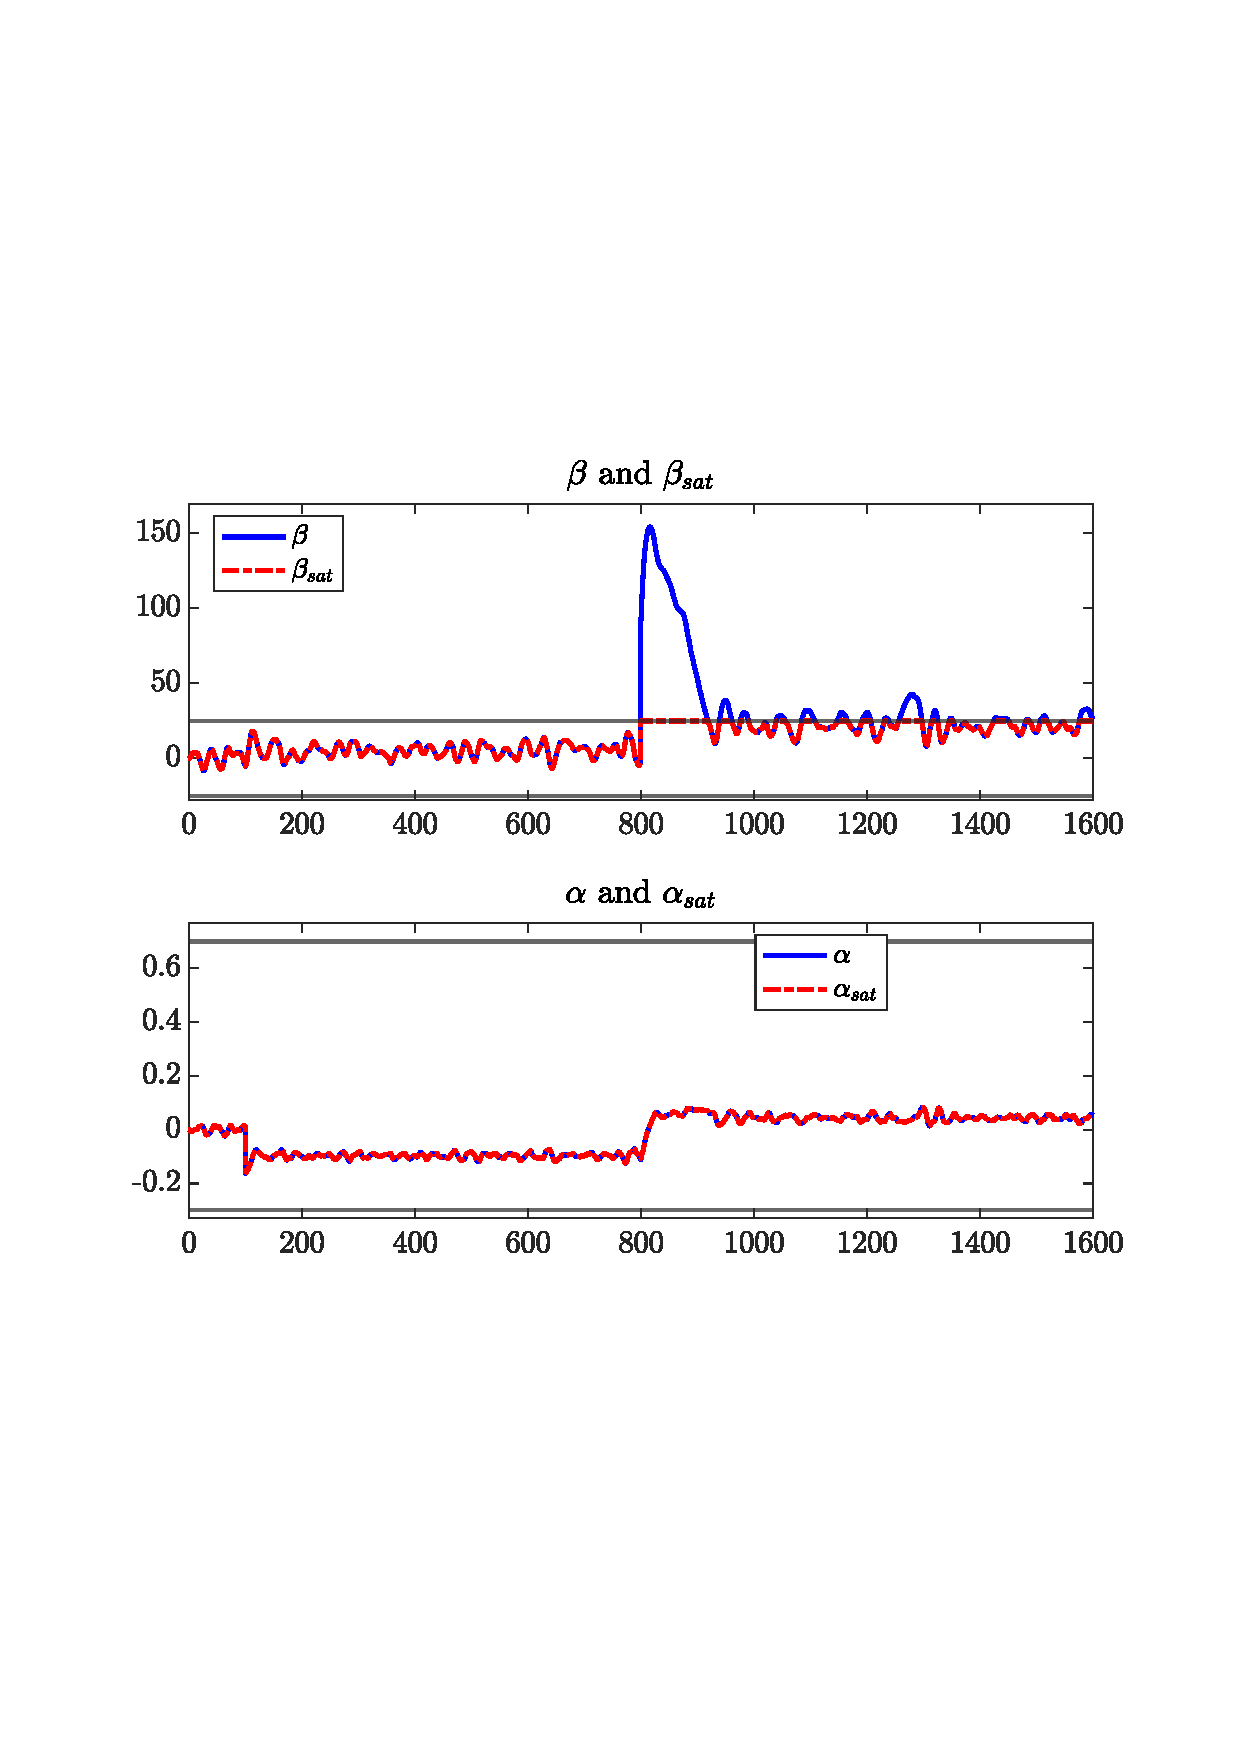
\includegraphics[width=1\linewidth, scale=1, trim=55 230 55 120,clip]{fig/Open_loop/exp_6_in.pdf}}
\\
\subcaptionbox{Relative error over time. \label{fig:app:cl_results:exp6:error}}[.7\textwidth]{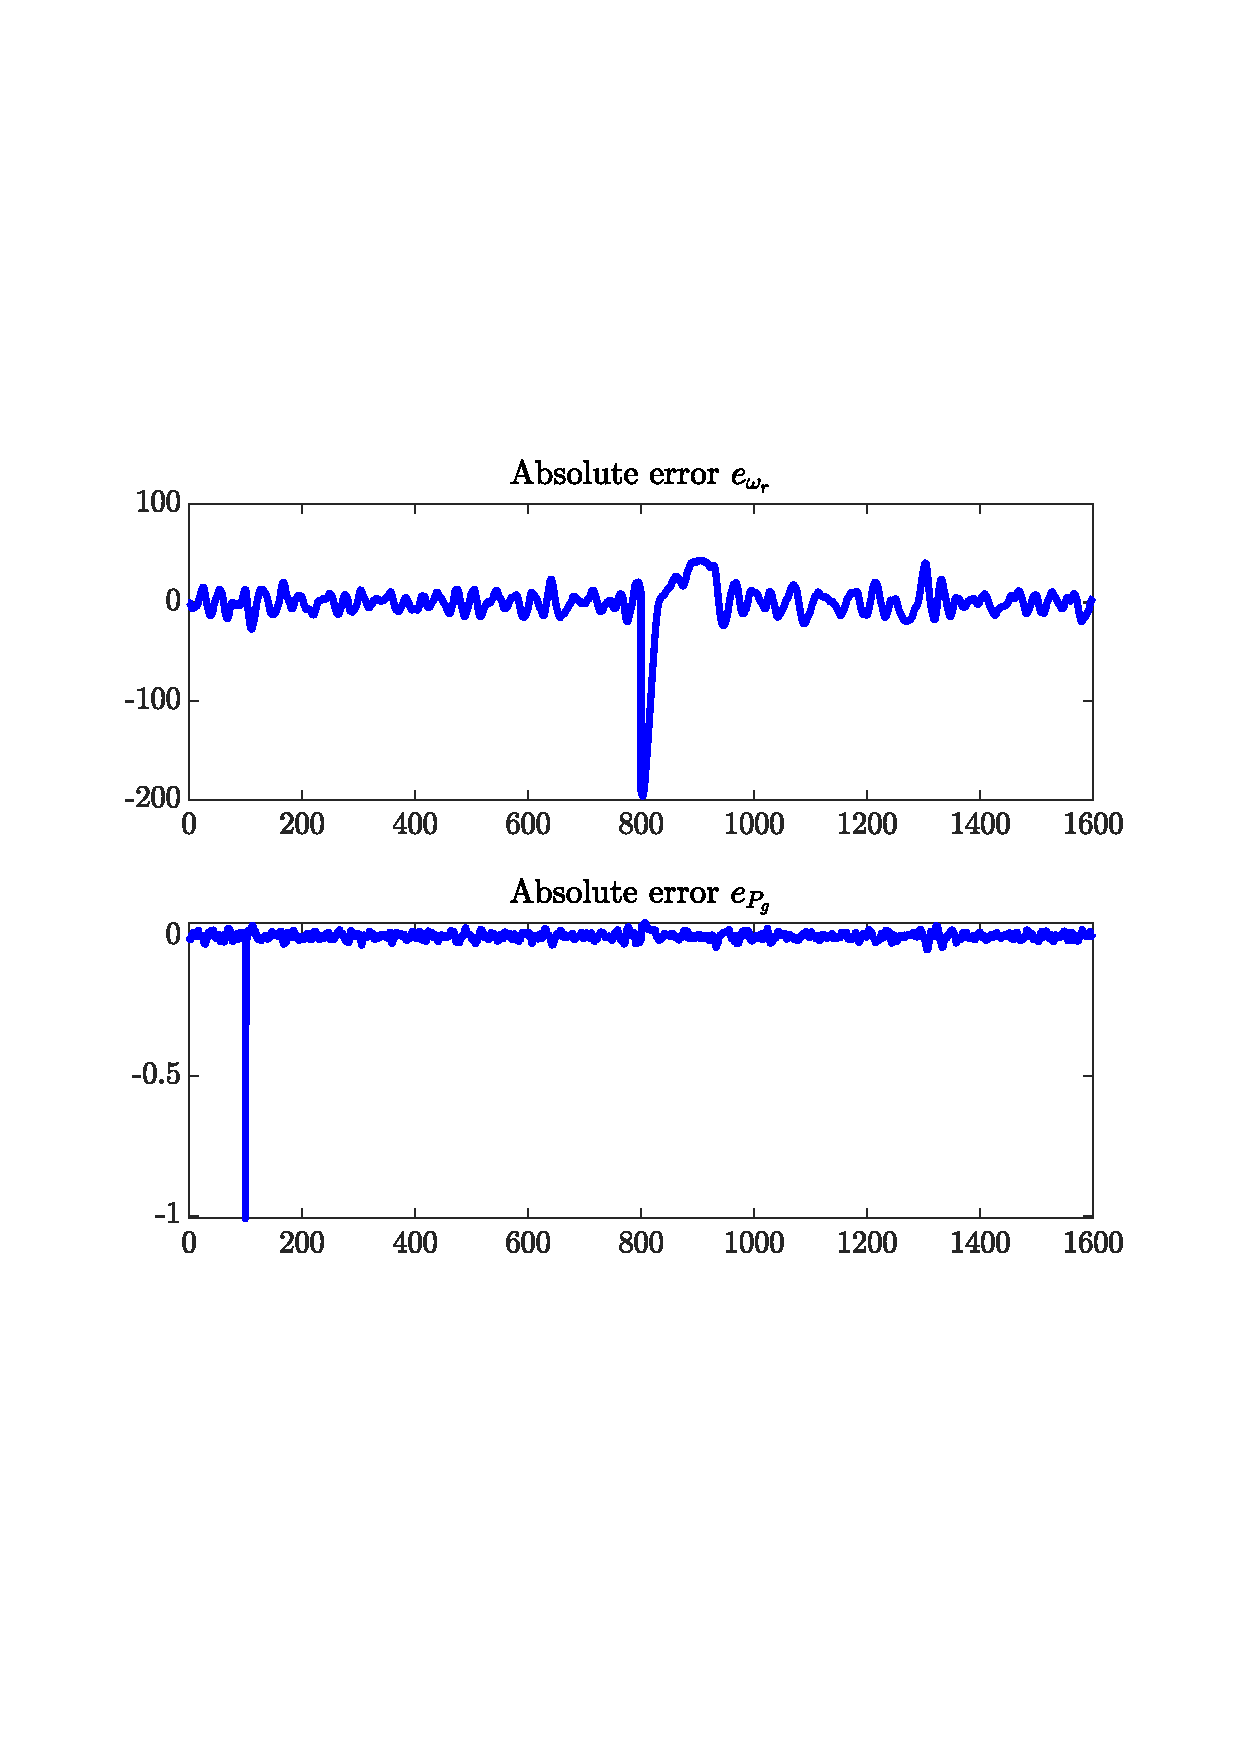
\includegraphics[width=1\linewidth, scale=1, trim=55 230 55 120,clip]{fig/Open_loop/exp_6_error.pdf}}
    \caption{Visualization of reference signal, the controller output and the absolute error}
    \label{fig:app:cl_results:exp6}
\end{figure}

\subsection{Experiment 7}

\begin{figure}[H]
    \centering

    \subcaptionbox{Wind disturbance, rotational speed of blade and power consumption over time \label{fig:app:cl_results:exp7:ref}}[.45\textwidth]{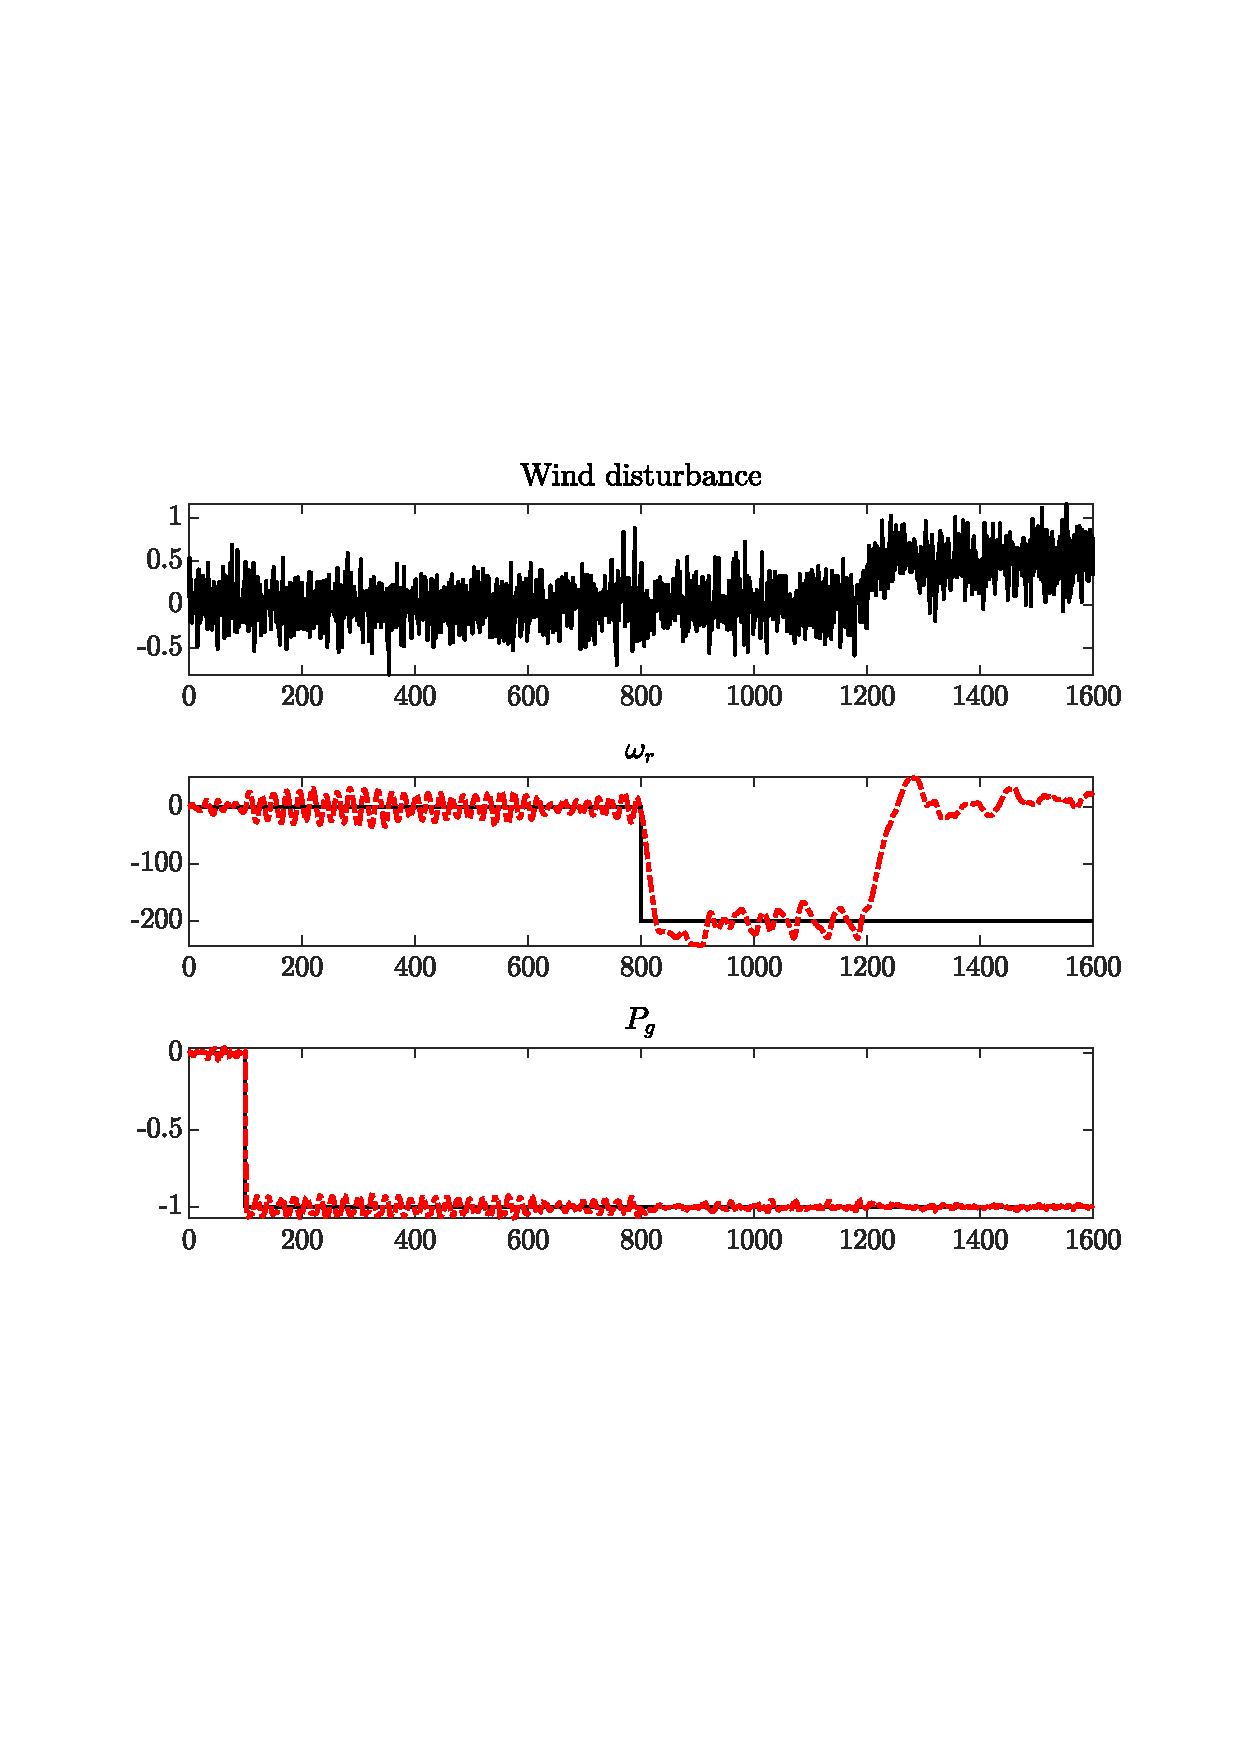
\includegraphics[width=1\linewidth, scale=1, trim=50 230 55 120,clip]{fig/Open_loop/exp_7_ref.pdf}}
%
    \subcaptionbox{Blade pitch angle and duty cycle over time before and after saturation. \label{fig:app:cl_results:exp7:in}}[.45\textwidth]{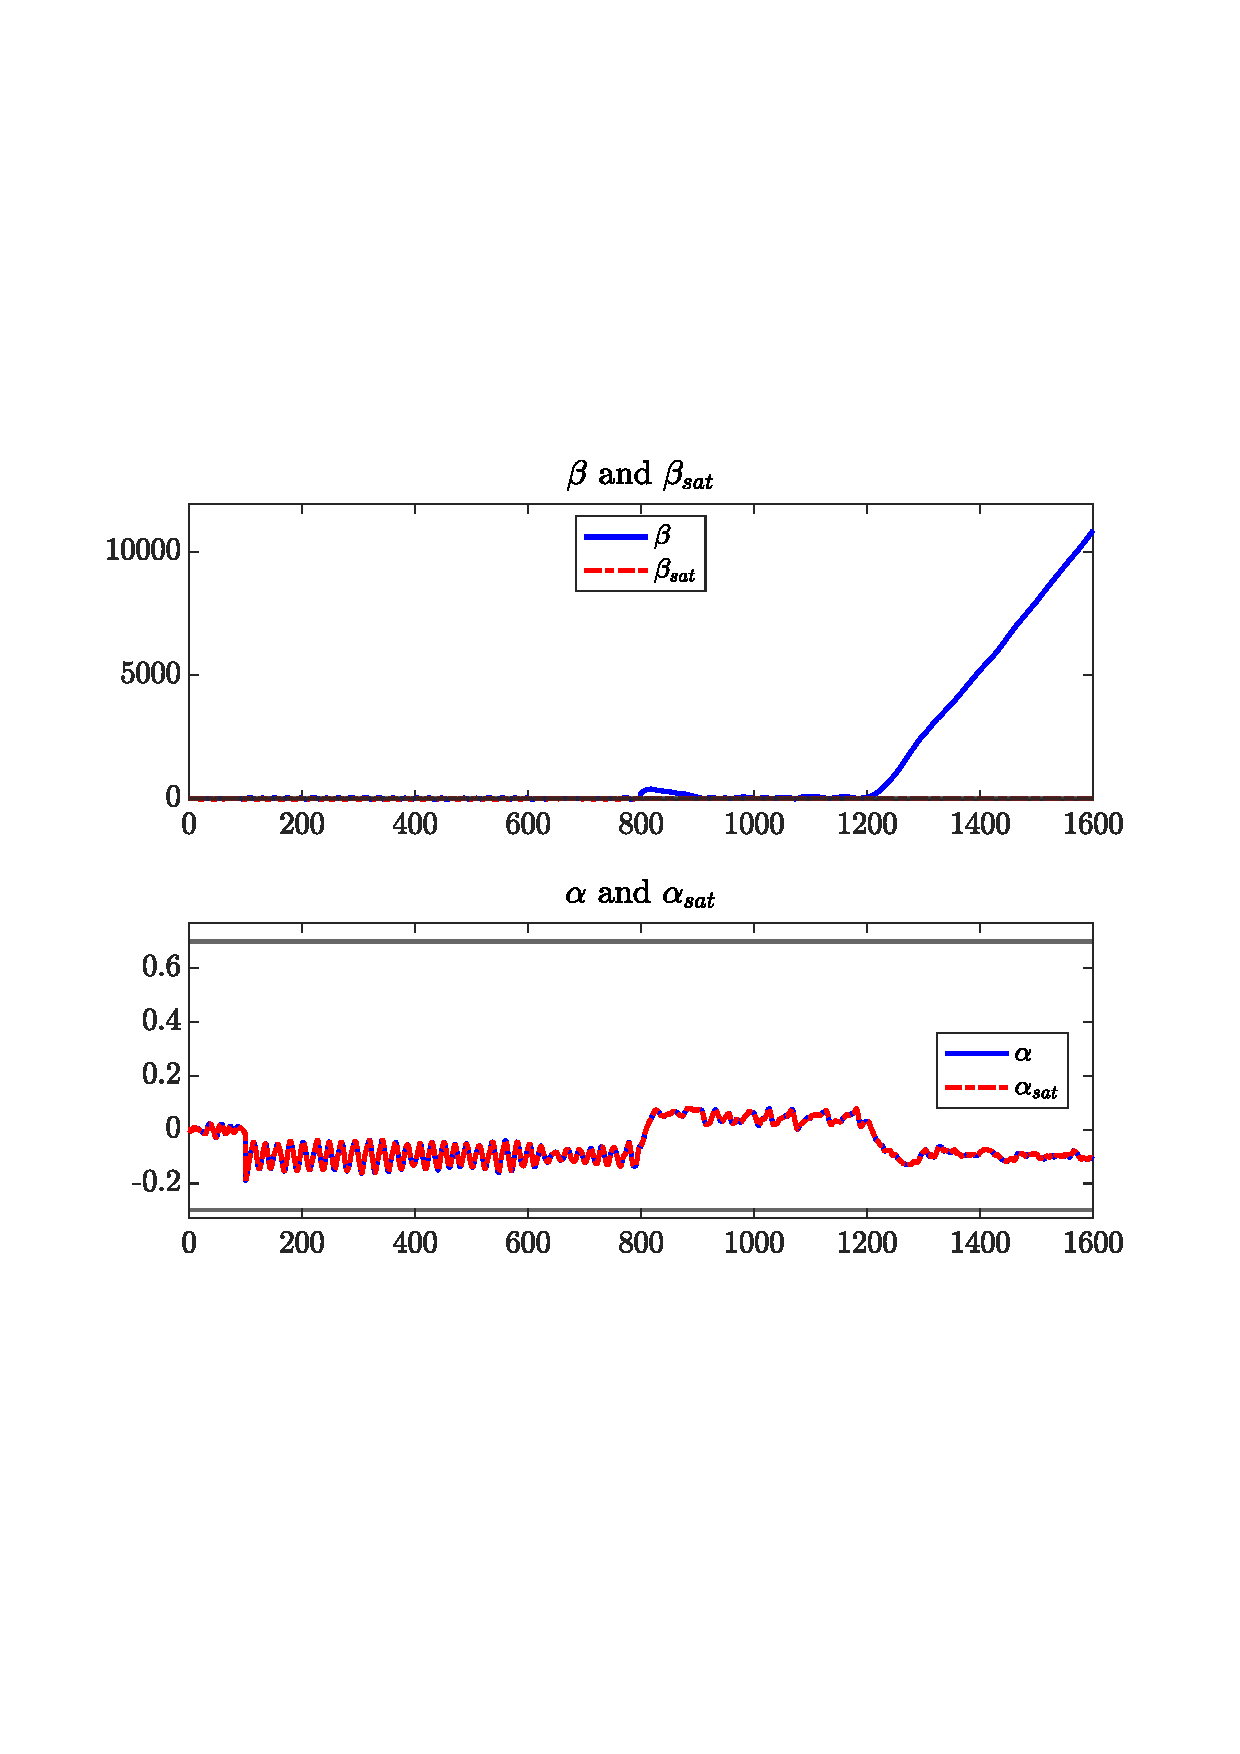
\includegraphics[width=1\linewidth, scale=1, trim=55 230 55 120,clip]{fig/Open_loop/exp_7_in.pdf}}
\\
\subcaptionbox{Relative error over time. \label{fig:app:cl_results:exp7:error}}[.7\textwidth]{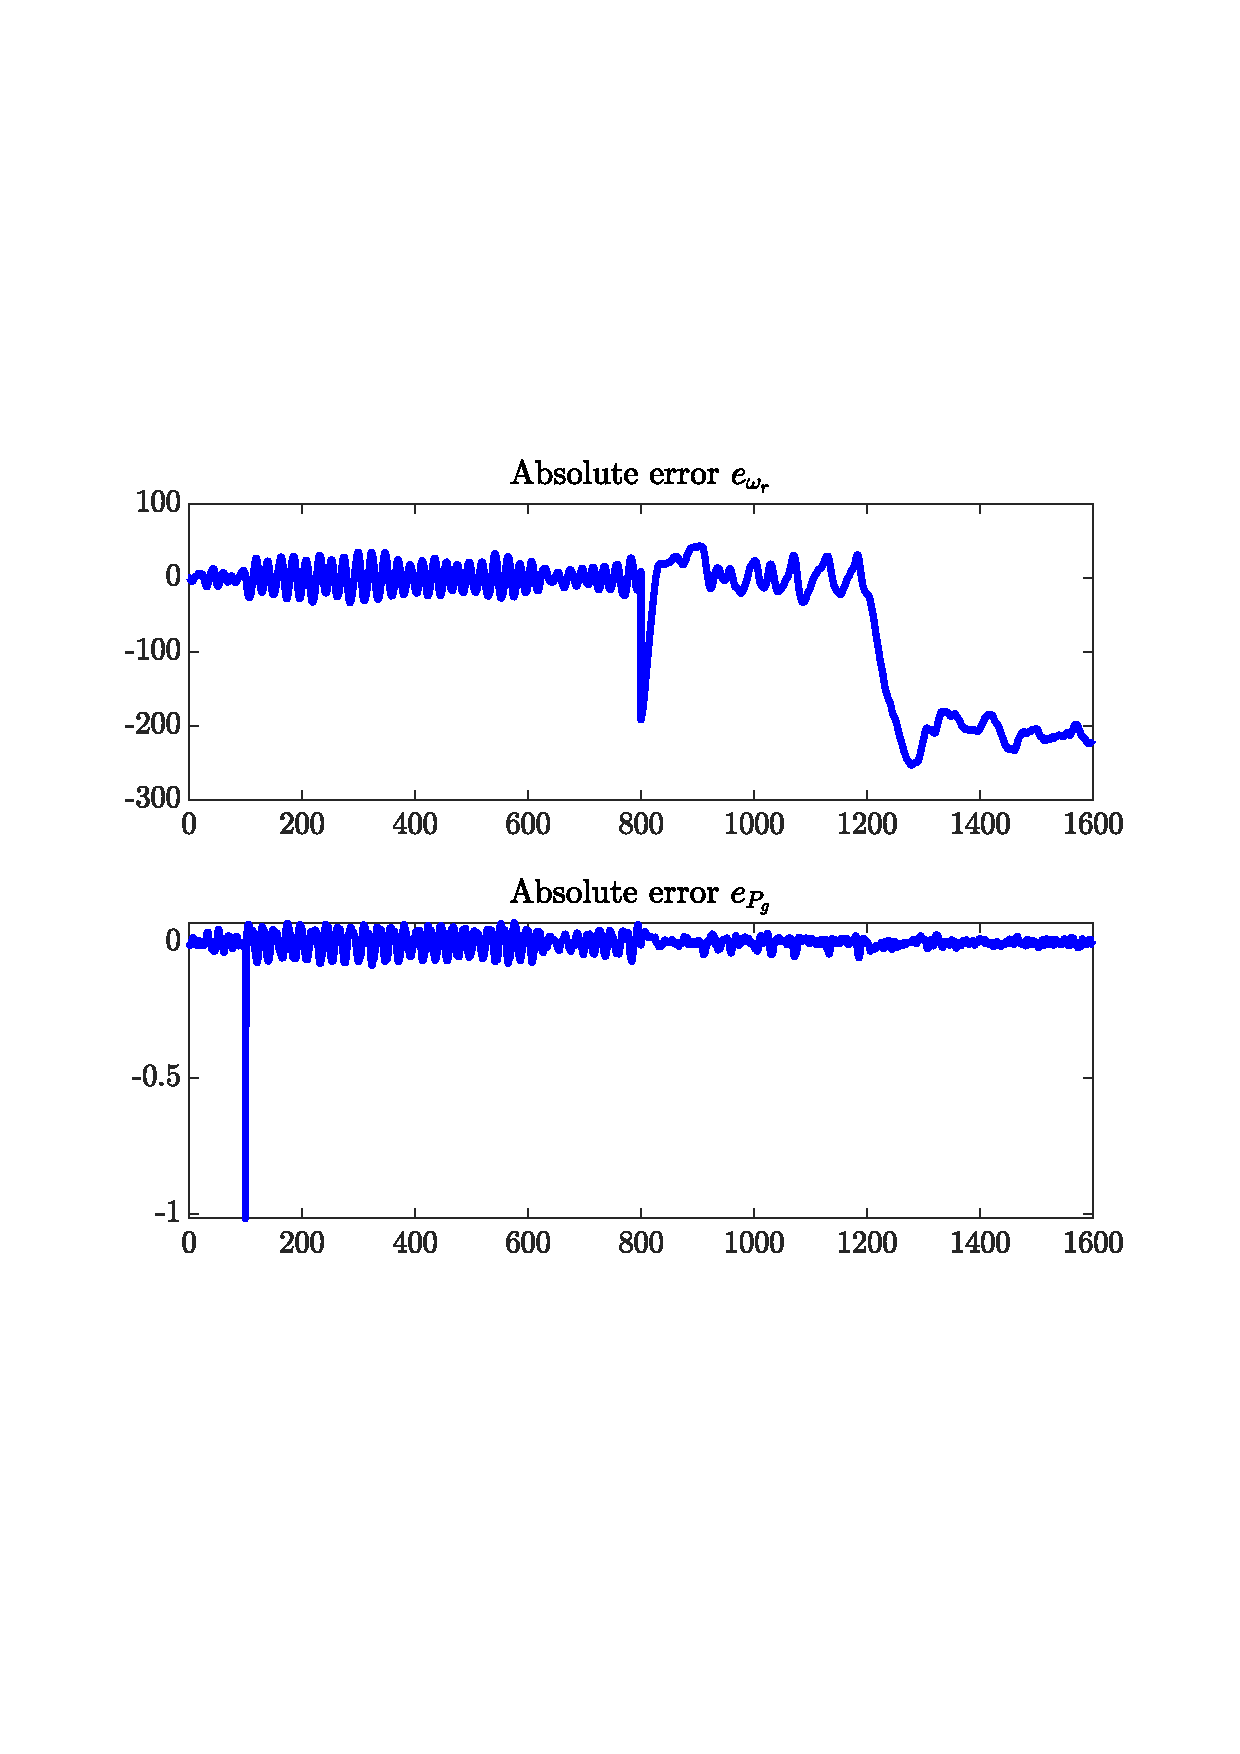
\includegraphics[width=1\linewidth, scale=1, trim=55 230 55 120,clip]{fig/Open_loop/exp_7_error.pdf}}
    \caption{Visualization of reference signal, the controller output and the absolute error}
    \label{fig:app:cl_results:exp7}
\end{figure}

\subsection{Experiment 8}

\begin{figure}[H]
    \centering

    \subcaptionbox{Wind disturbance, rotational speed of blade and power consumption over time \label{fig:app:cl_results:exp8:ref}}[.45\textwidth]{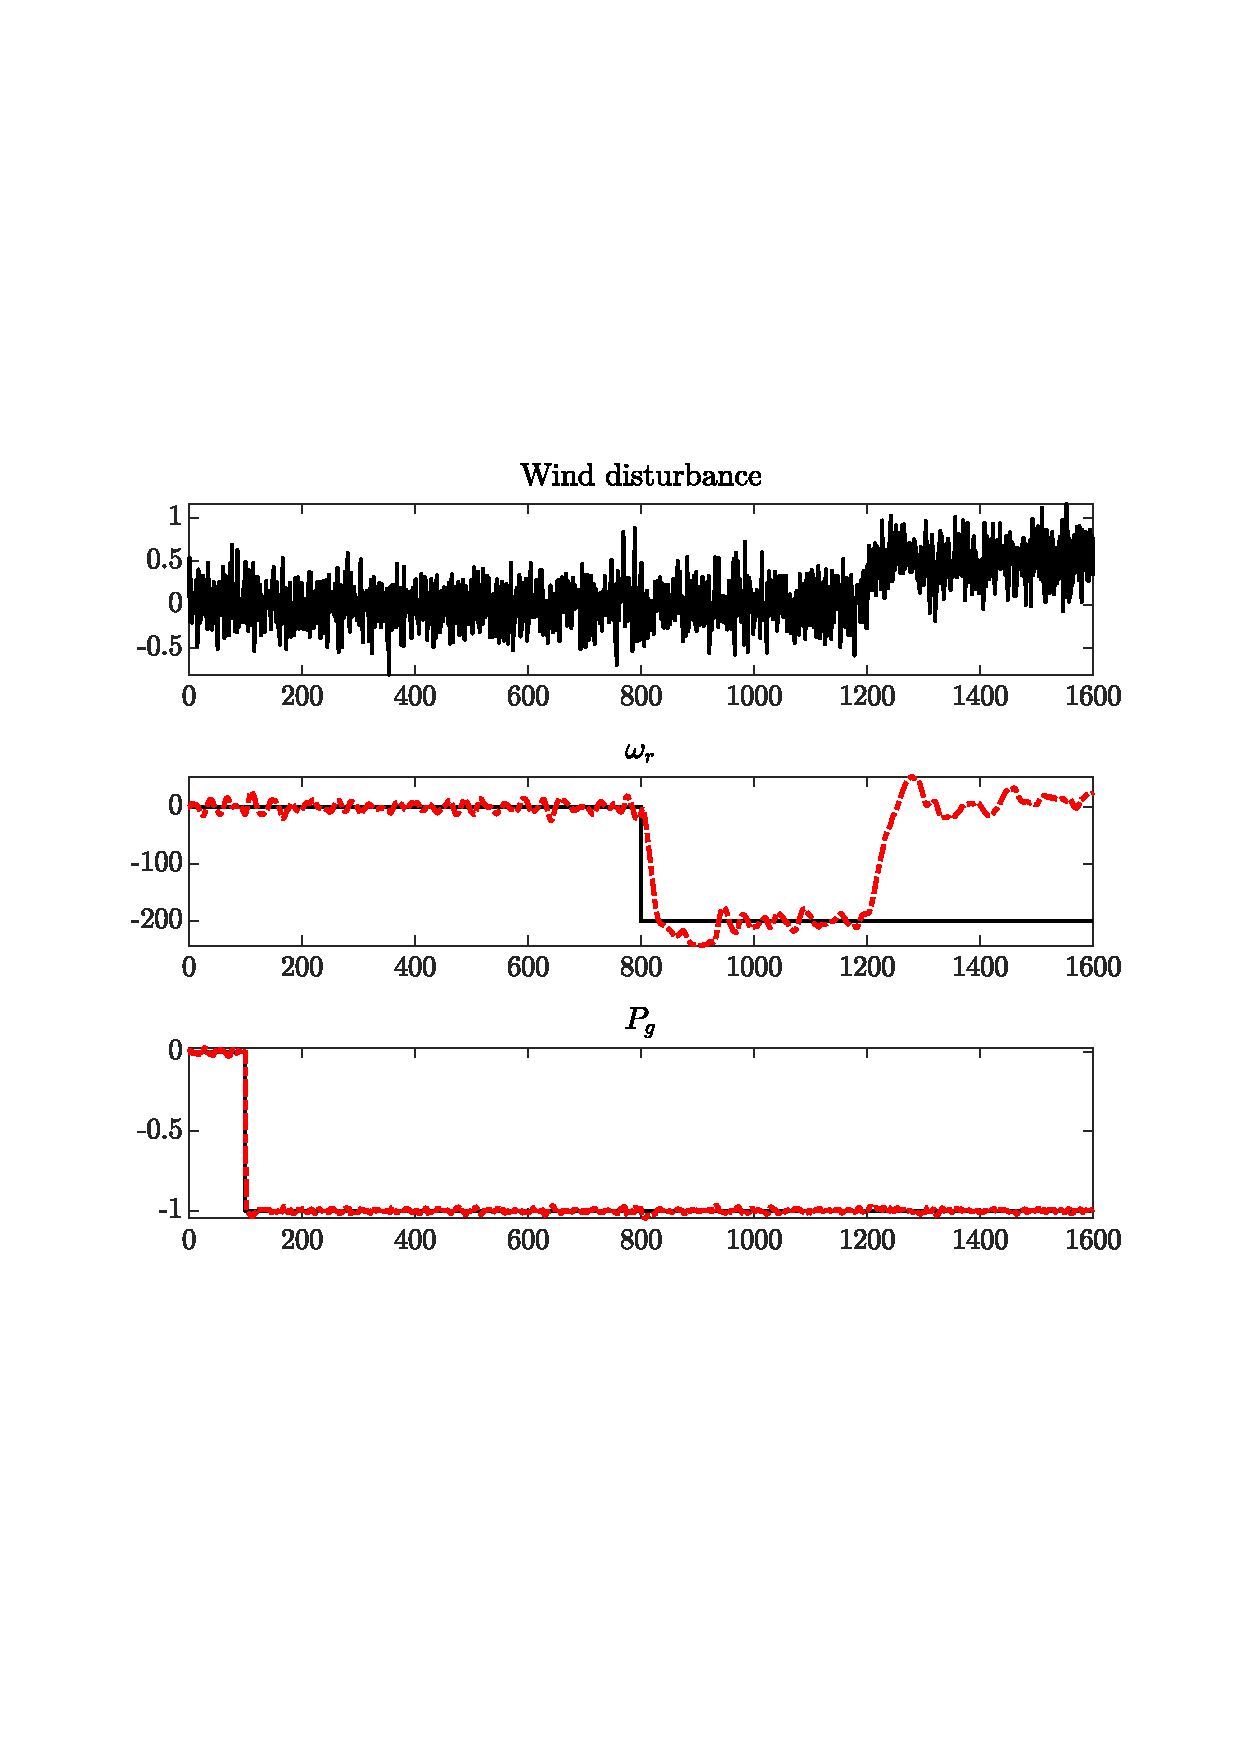
\includegraphics[width=1\linewidth, scale=1, trim=55 230 55 120,clip]{fig/Open_loop/exp_8_ref.pdf}}
%
    \subcaptionbox{Blade pitch angle and duty cycle over time before and after saturation. \label{fig:app:cl_results:exp8:in}}[.45\textwidth]{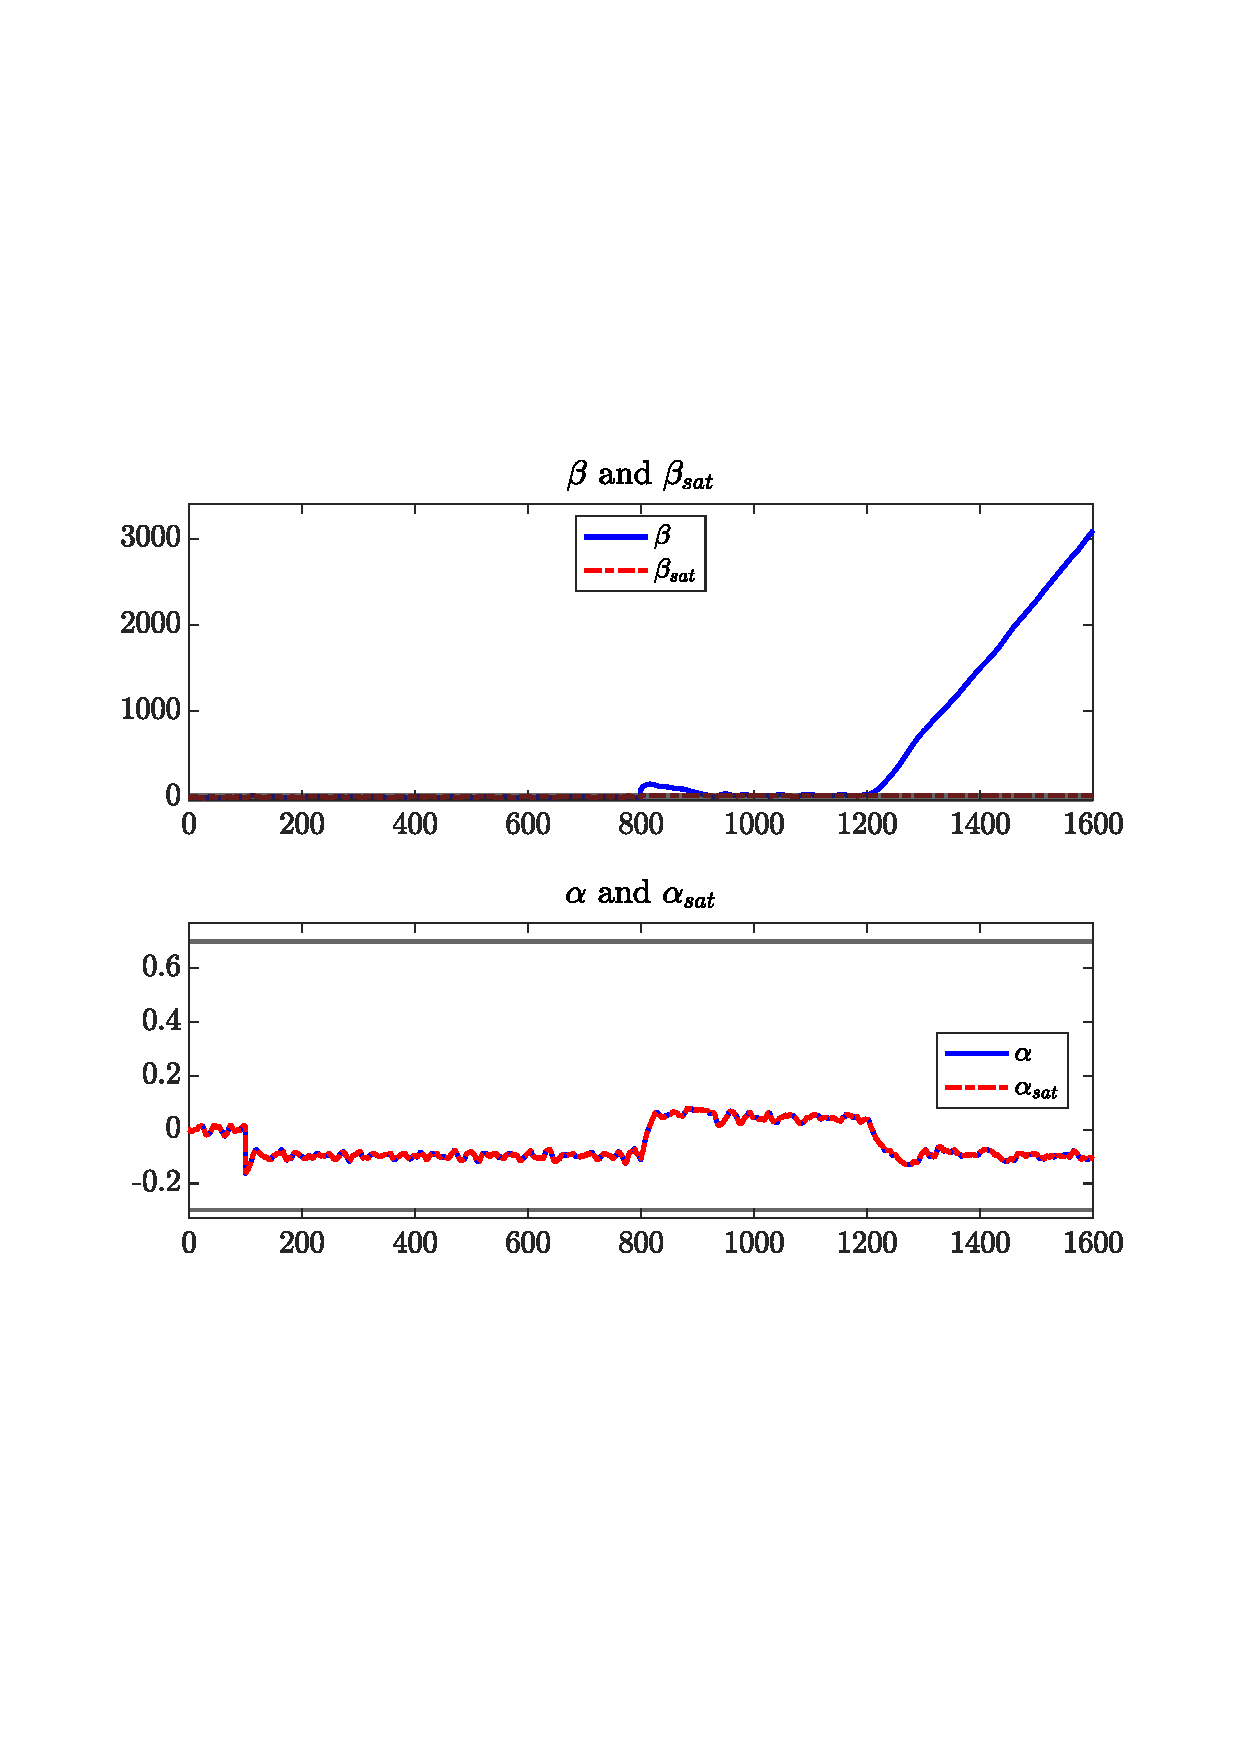
\includegraphics[width=1\linewidth, scale=1, trim=55 230 55 120,clip]{fig/Open_loop/exp_8_in.pdf}}
\\
\subcaptionbox{Relative error over time. \label{fig:app:cl_results:exp8:error}}[.7\textwidth]{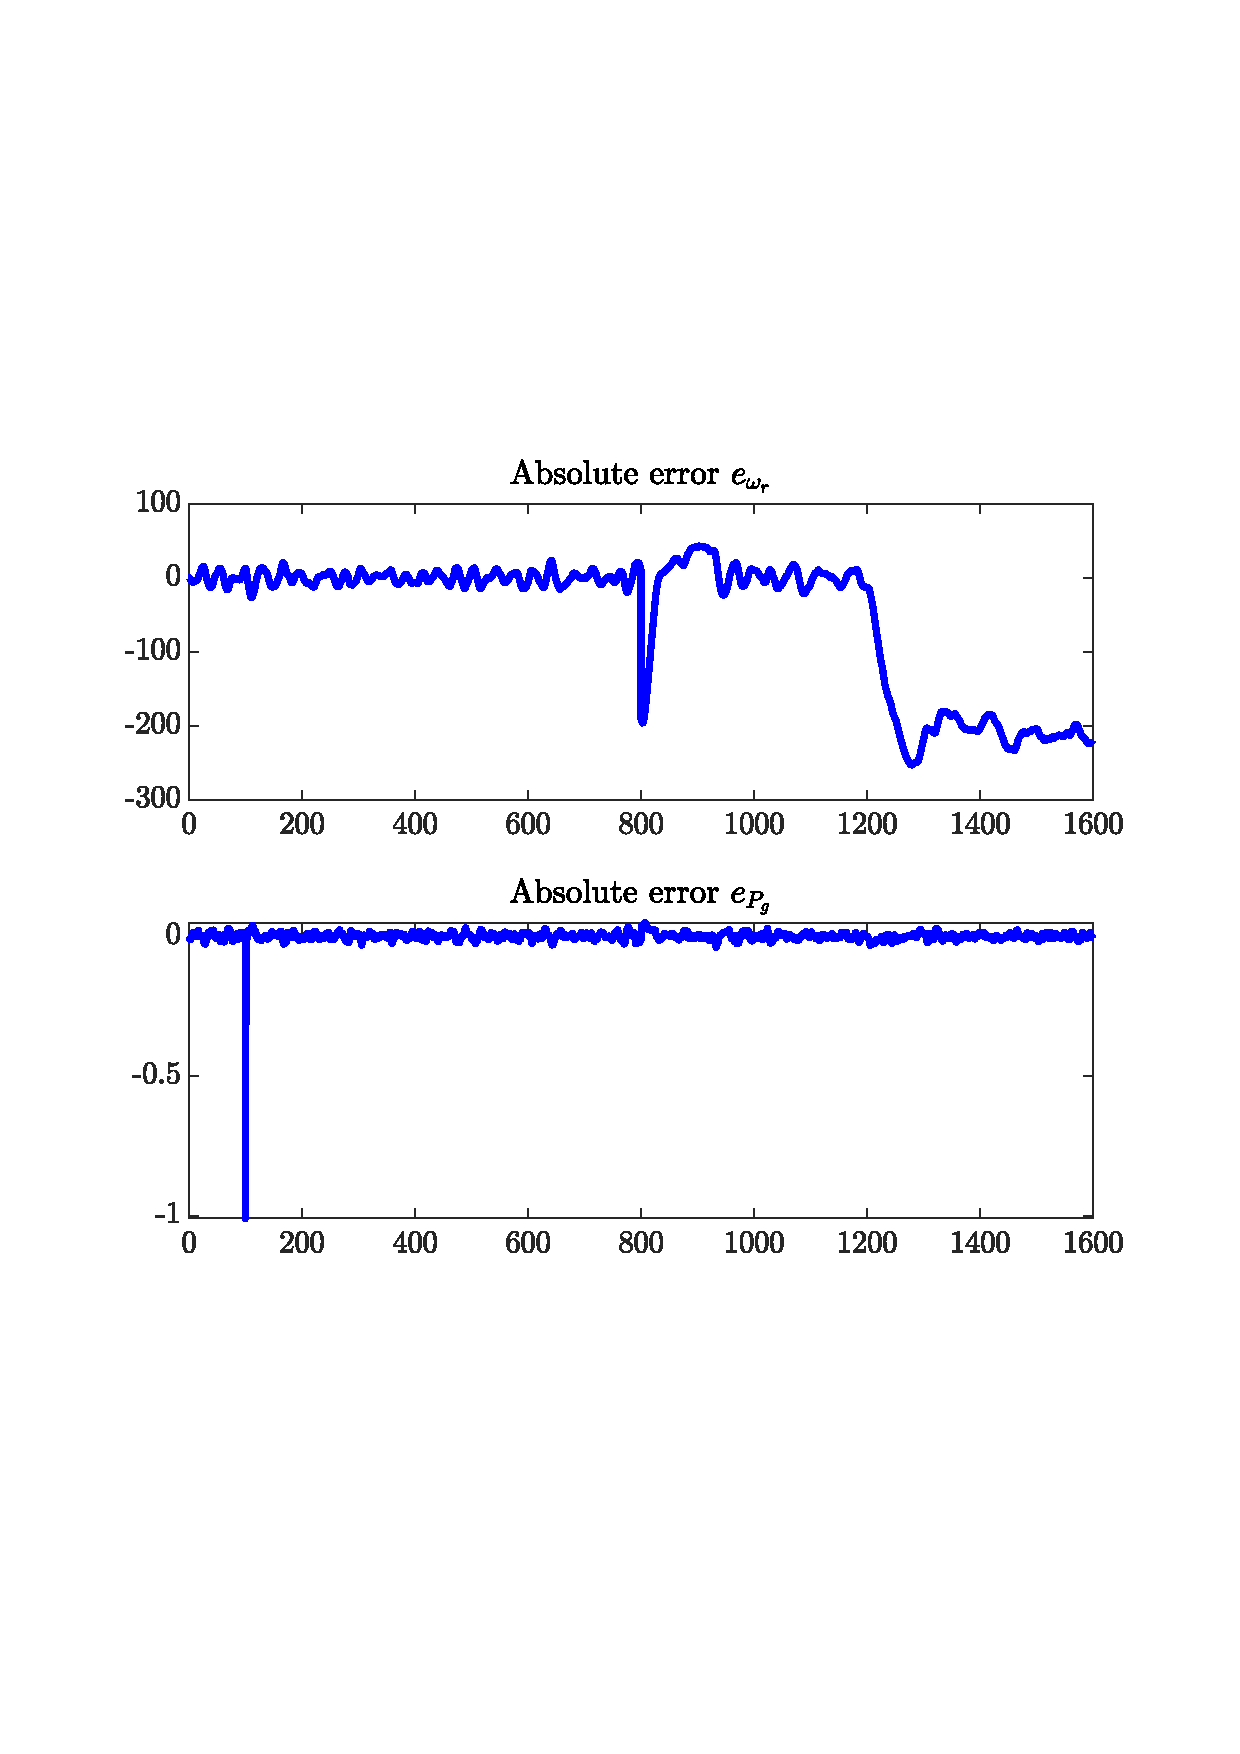
\includegraphics[width=1\linewidth, scale=1, trim=55 230 55 120,clip]{fig/Open_loop/exp_8_error.pdf}}
    \caption{Visualization of reference signal, the controller output and the absolute error}
    \label{fig:app:cl_results:exp8}
\end{figure}


\subsection{Experiment 9}

\begin{figure}[H]
    \centering

    \subcaptionbox{Wind disturbance, rotational speed of blade and power consumption over time \label{fig:app:cl_results:exp9:ref}}[.45\textwidth]{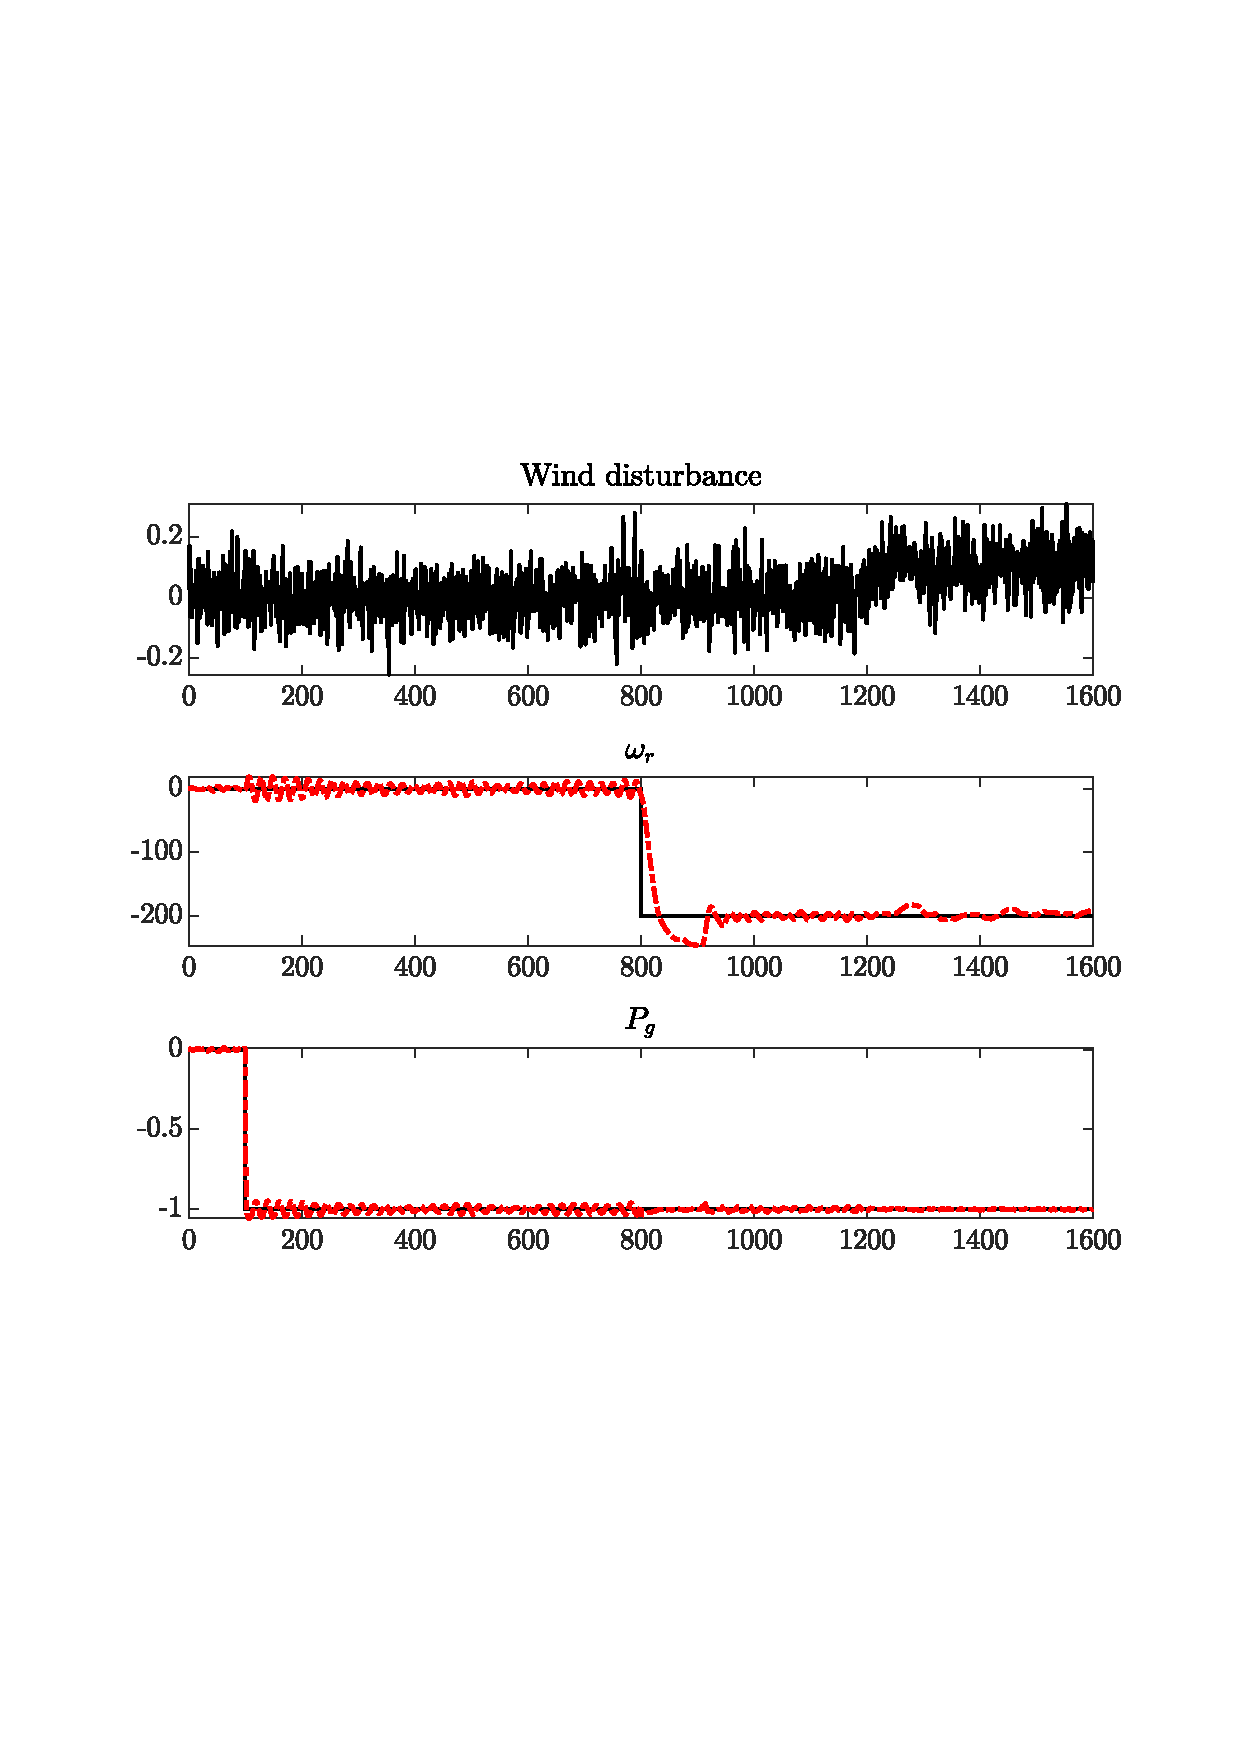
\includegraphics[width=1\linewidth, scale=1, trim=55 230 55 120,clip]{fig/Open_loop/exp_9_ref.pdf}}
%
    \subcaptionbox{Blade pitch angle and duty cycle over time before and after saturation. \label{fig:app:cl_results:exp9:in}}[.45\textwidth]{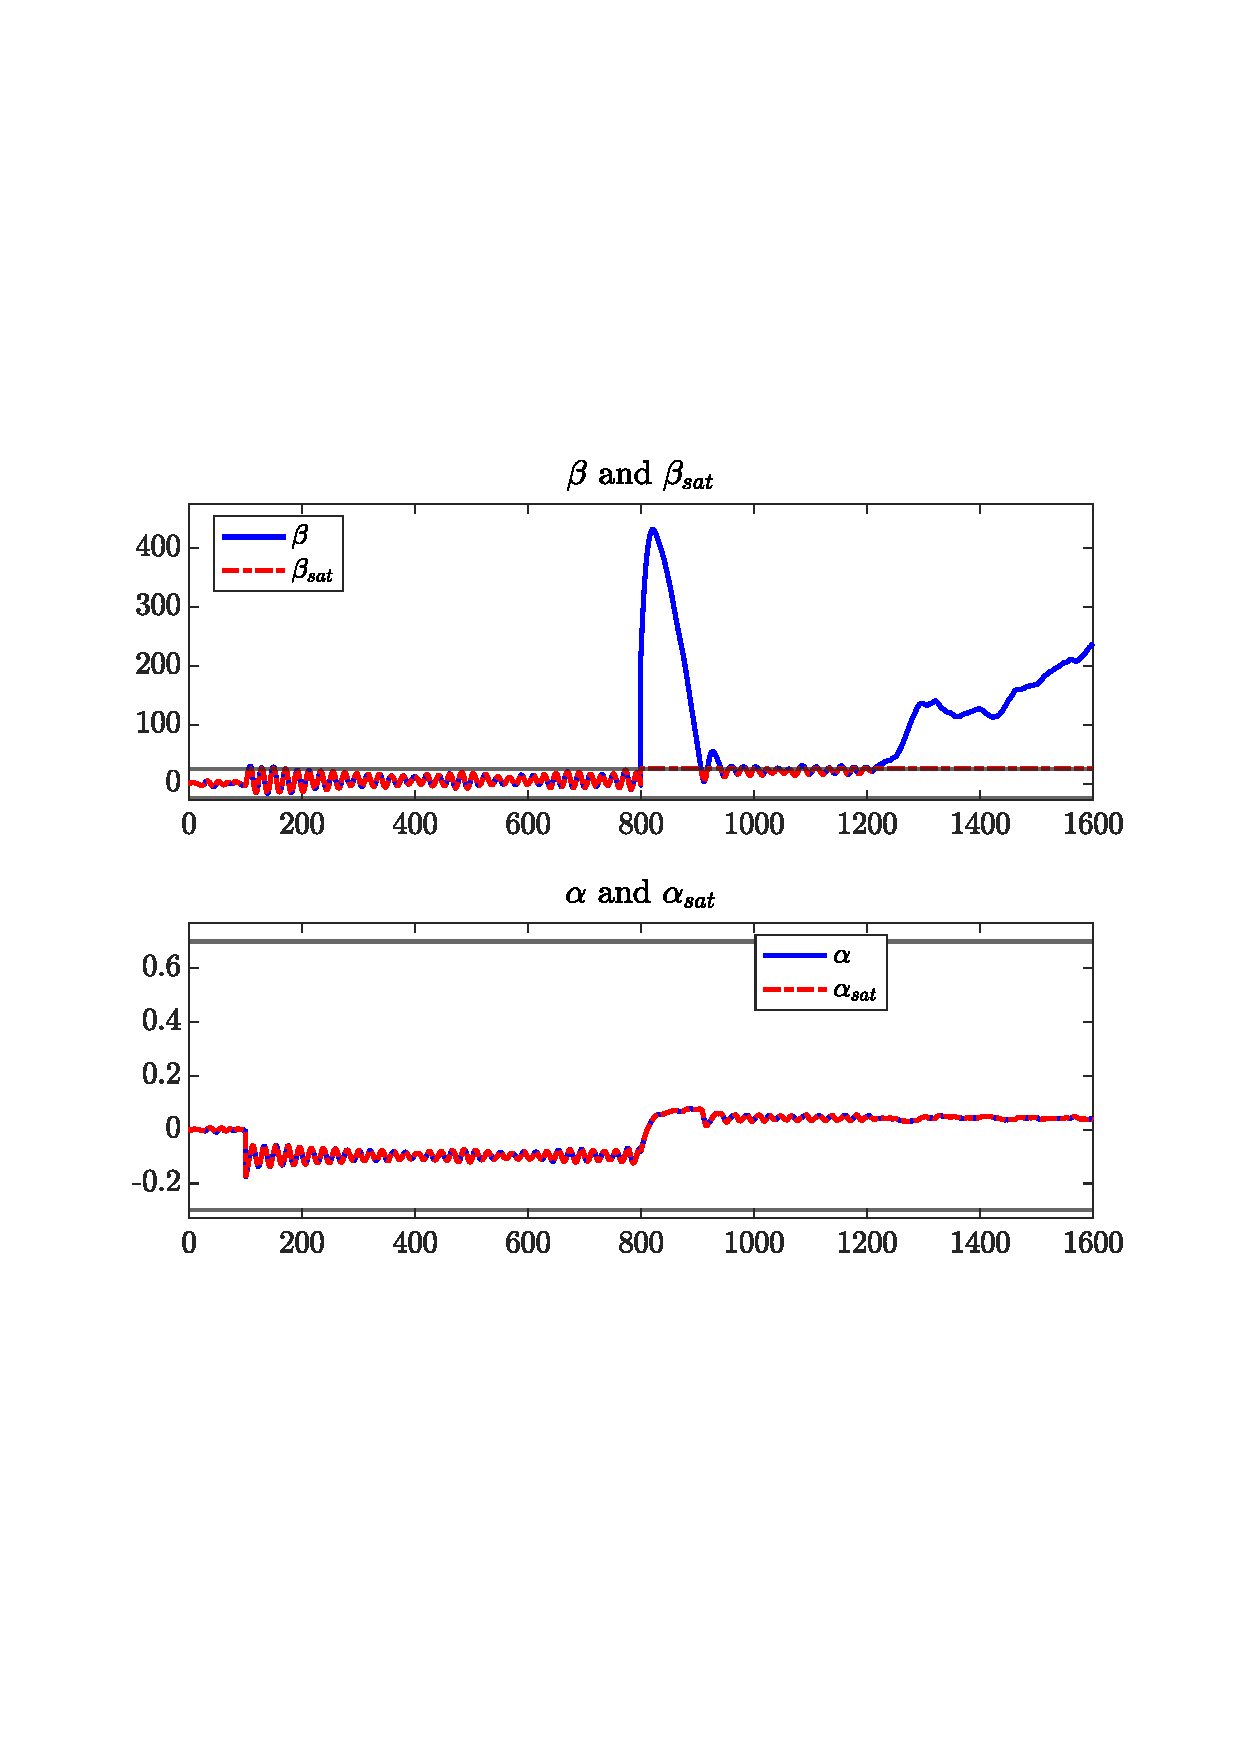
\includegraphics[width=1\linewidth, scale=1, trim=55 230 55 120,clip]{fig/Open_loop/exp_9_in.pdf}}
\\
\subcaptionbox{Relative error over time. \label{fig:app:cl_results:exp9:error}}[.7\textwidth]{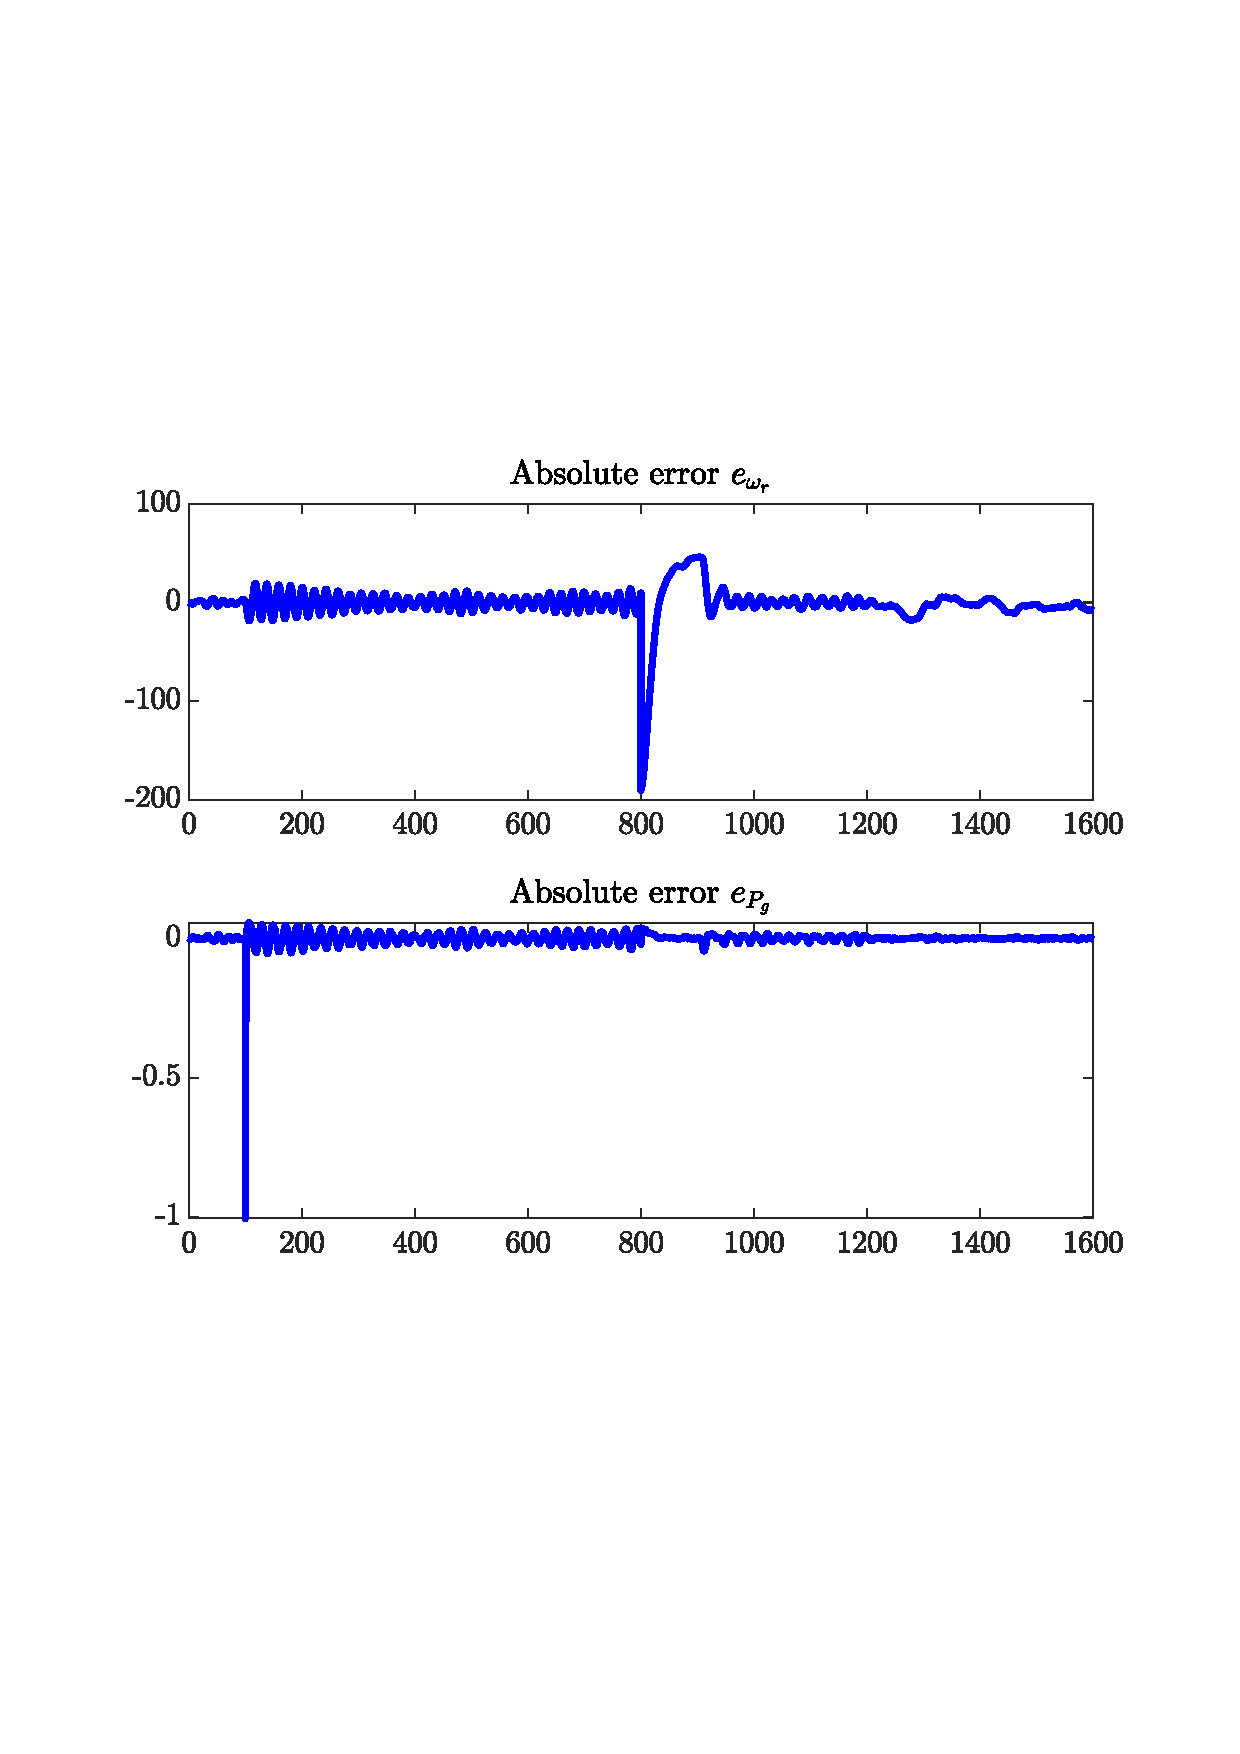
\includegraphics[width=1\linewidth, scale=1, trim=55 230 55 120,clip]{fig/Open_loop/exp_9_error.pdf}}
    \caption{Visualization of reference signal, the controller output and the absolute error}
    \label{fig:app:cl_results:exp9}
\end{figure}


\subsection{Experiment 10}

\begin{figure}[H]
    \centering

    \subcaptionbox{Wind disturbance, rotational speed of blade and power consumption over time \label{fig:app:cl_results:exp10:ref}}[.45\textwidth]{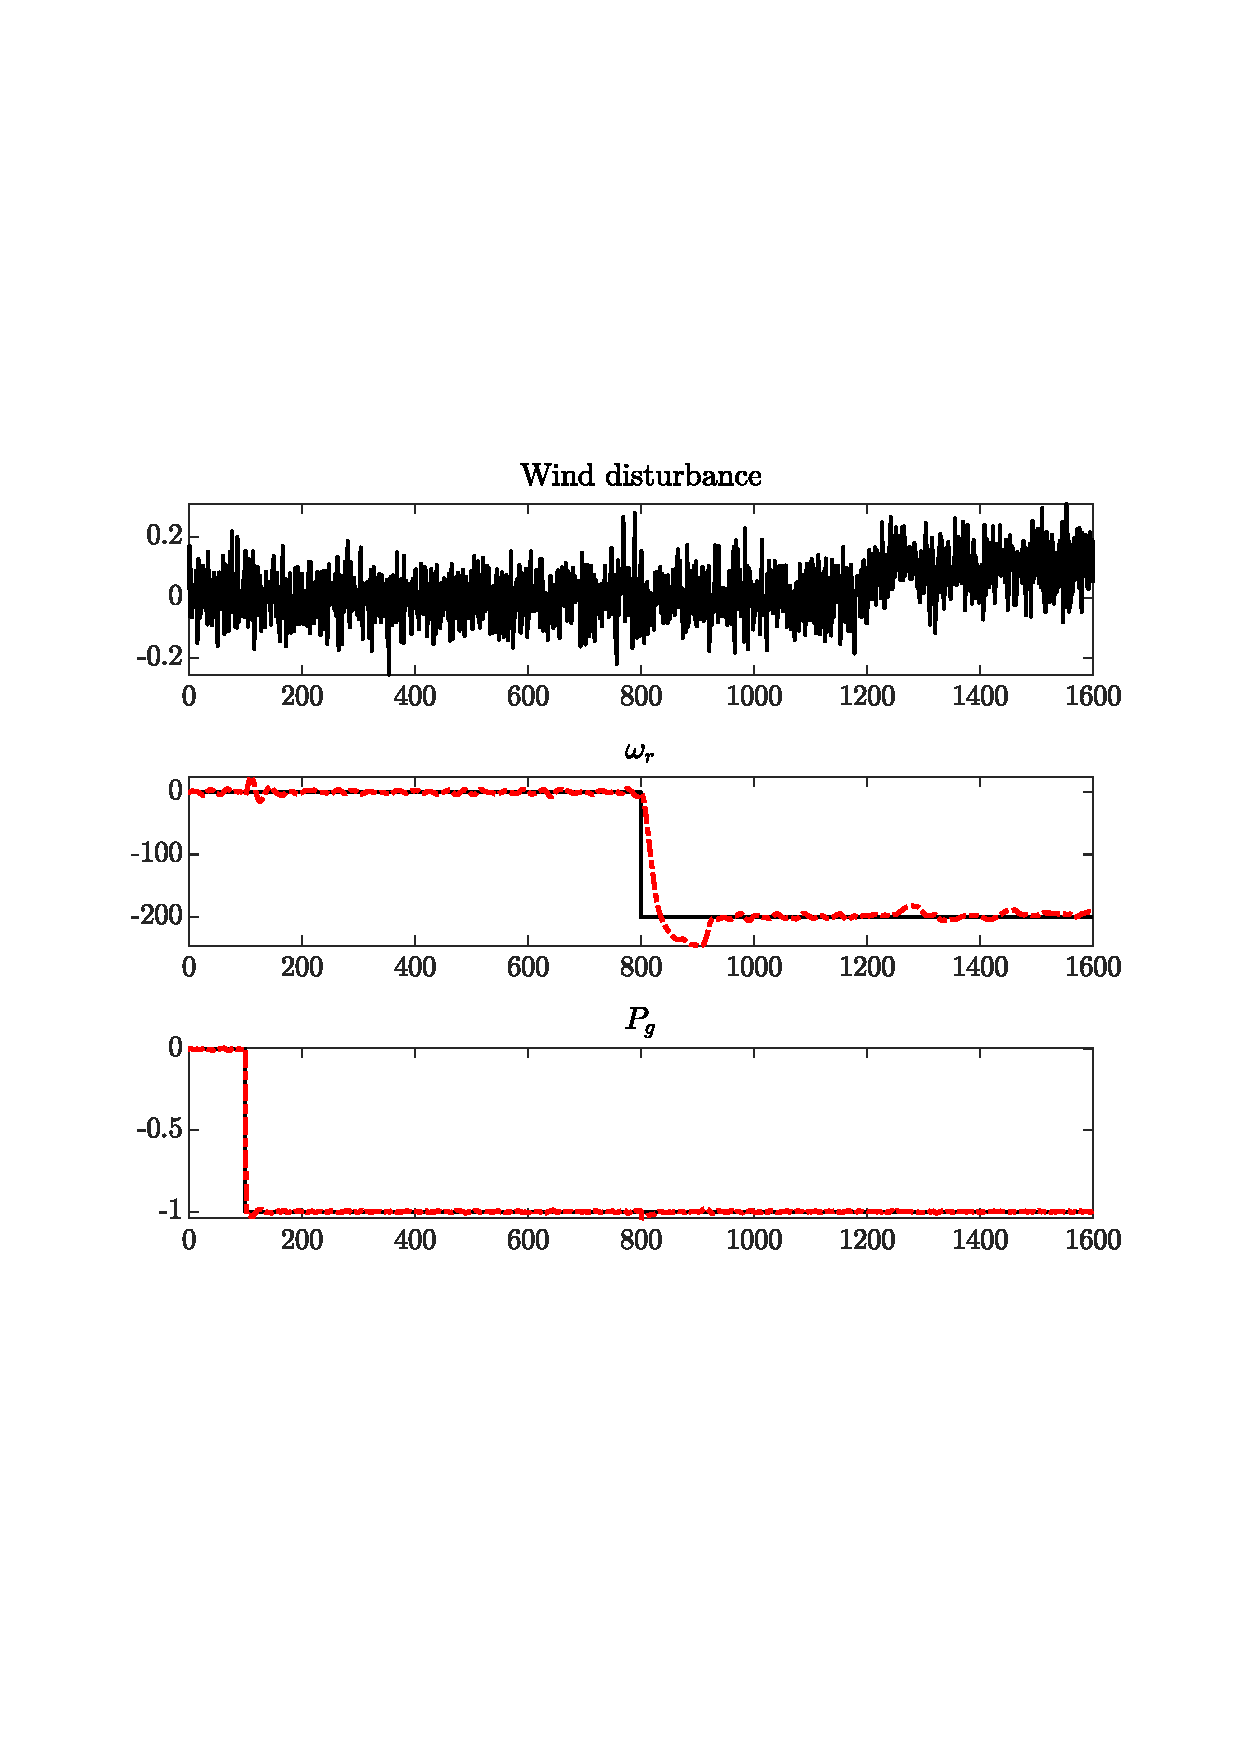
\includegraphics[width=1\linewidth, scale=1, trim=55 230 55 120,clip]{fig/Open_loop/exp_10_ref.pdf}}
%
    \subcaptionbox{Blade pitch angle and duty cycle over time before and after saturation. \label{fig:app:cl_results:exp10:in}}[.45\textwidth]{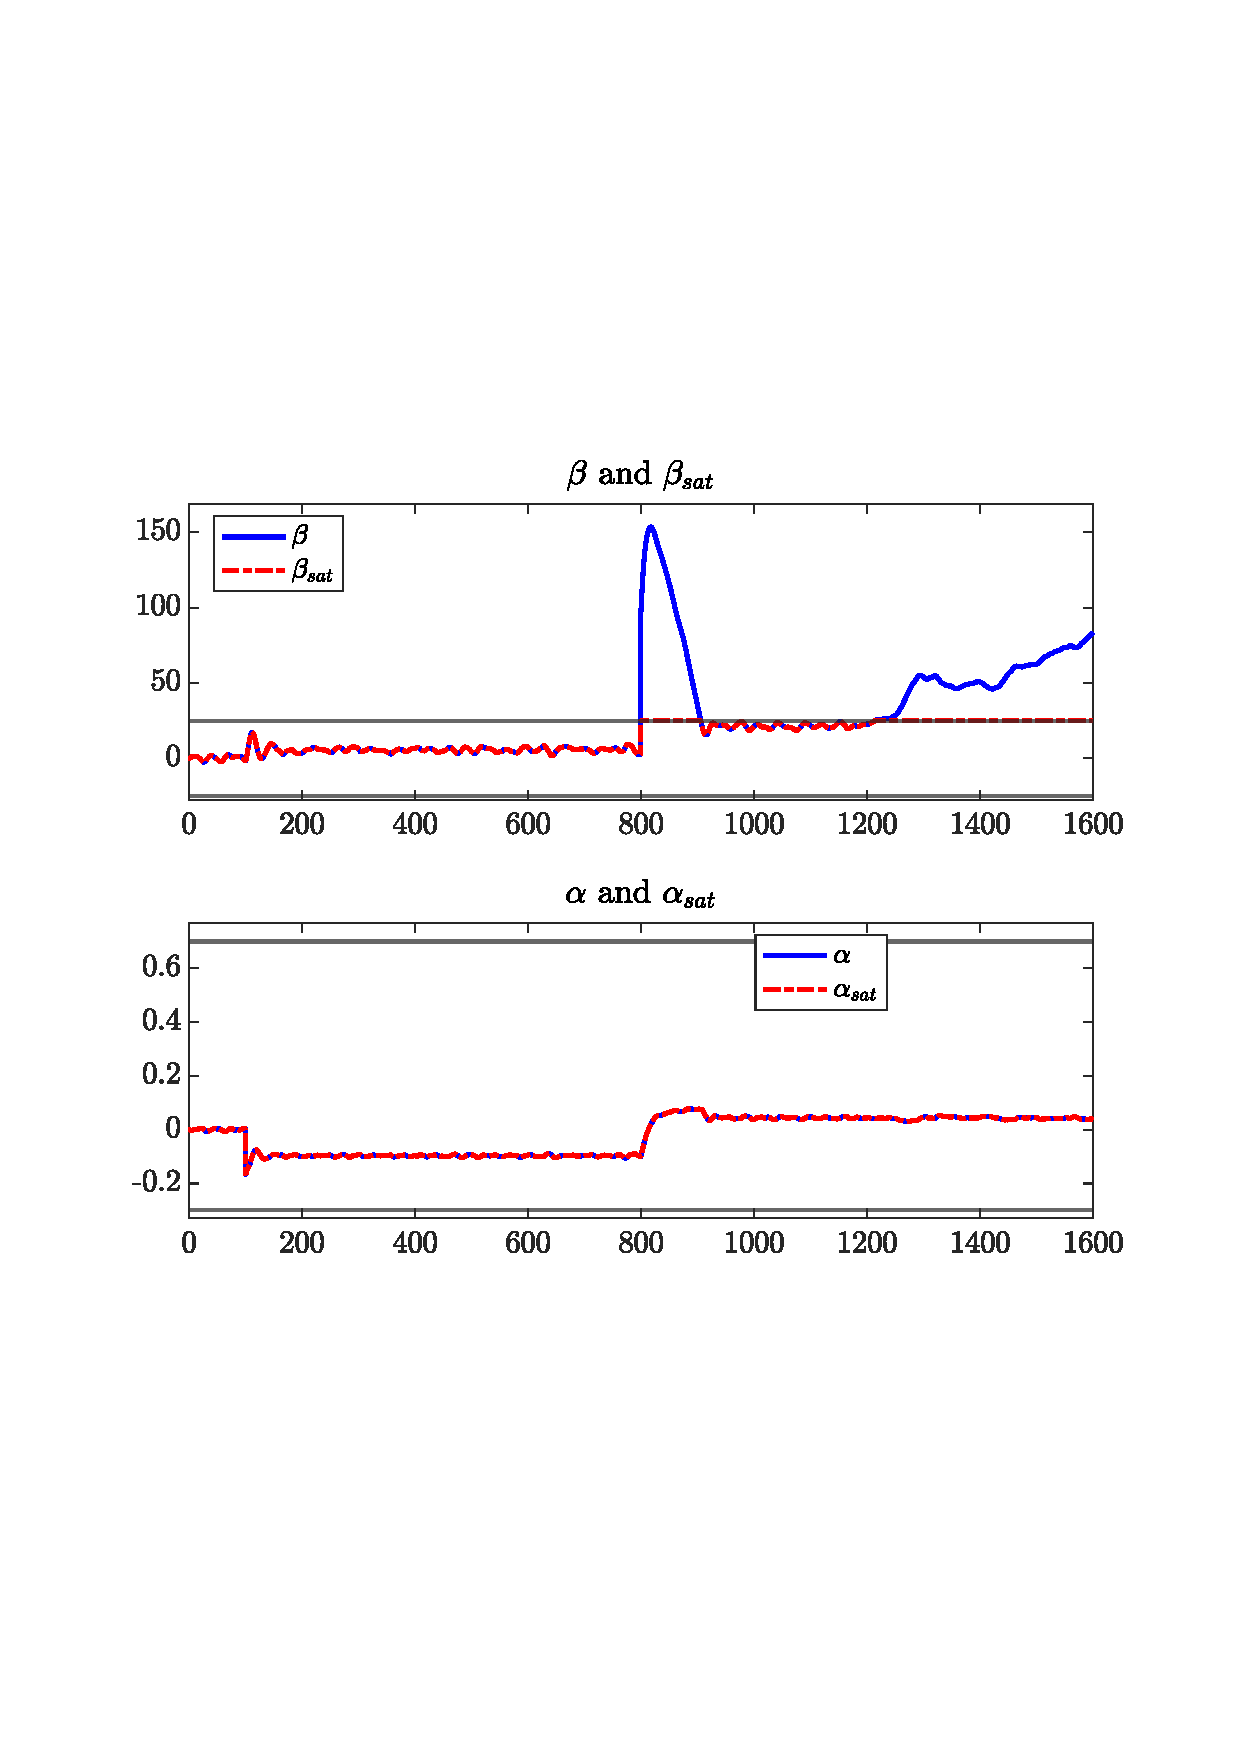
\includegraphics[width=1\linewidth, scale=1, trim=55 230 55 120,clip]{fig/Open_loop/exp_10_in.pdf}}
\\
\subcaptionbox{Relative error over time. \label{fig:app:cl_results:exp10:error}}[.7\textwidth]{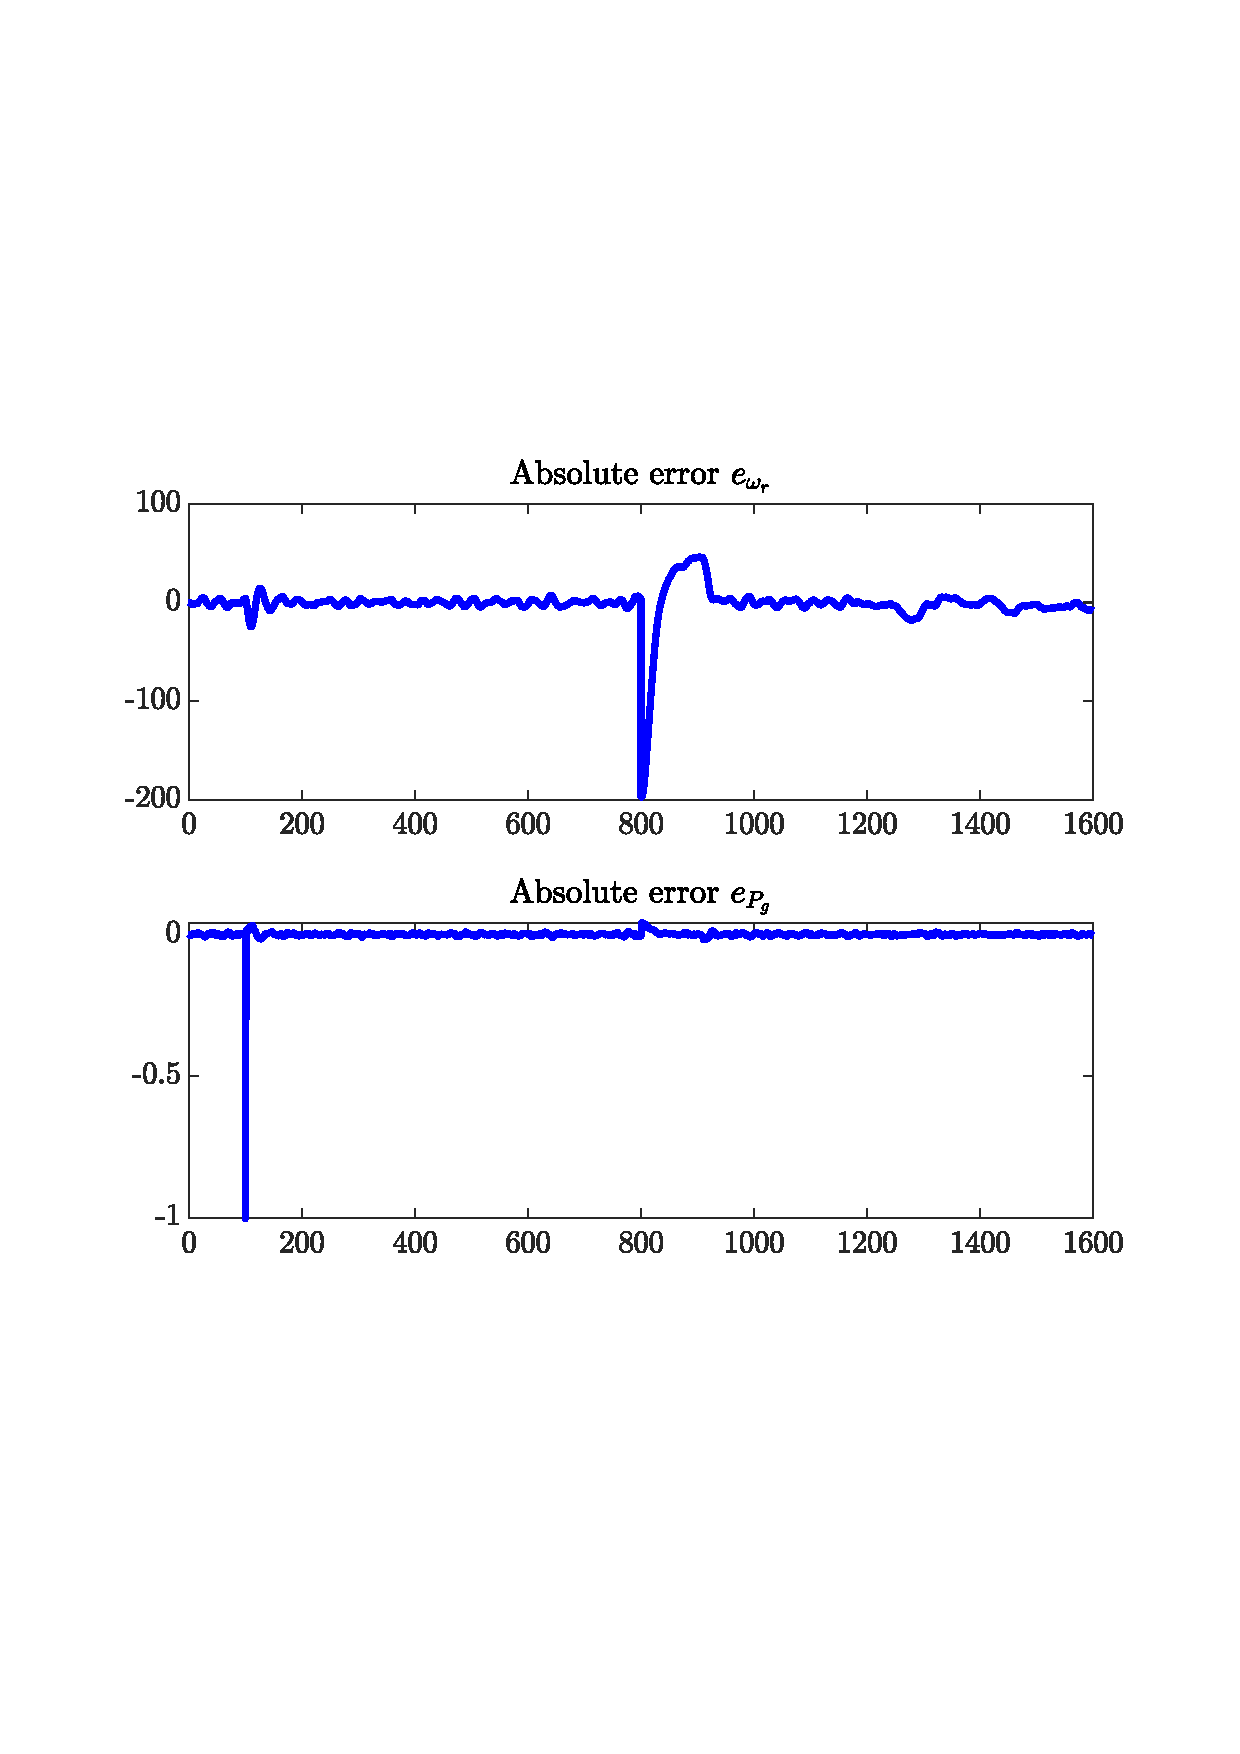
\includegraphics[width=1\linewidth, scale=1, trim=55 230 55 120,clip]{fig/Open_loop/exp_10_error.pdf}}
    \caption{Visualization of reference signal, the controller output and the absolute error}
    \label{fig:app:cl_results:exp10}
\end{figure}